\section{The Anonymous Face and Hand Tracking Panda}
When reviewing and testing the Anonymous Face Tracking Panda prototype, we found that the virtual avatar's ability to express themselves was limited by the lack of hand movement, which made it seem unrealistic and similar to a puppet acting. Through this finding, we questioned if the addition of hand tracking would affect or not the ability to elicit the same emotional response as human-to-human interactions (\textbf{RQ\textsubscript{1}}), and if it would help increase interactants' verbal self-disclosure or not (\textbf{RQ\textsubscript{2}}).

When people speak, they typically make spontaneous hand motions that occur in synchronization with speech and naturally accompany all spoken communication; such movements are known as gestures \cite{CLO20}. Gestures serve a diverse range of purposes in communication, learning, and comprehension for those who see them as well as those who make them. Gestures are particularly successful when they resemble the thought they represent, giving them an advantage over words since they offer relevant and distinct information while reflecting the speaker's underlying knowledge and experiences \cite{CLO20, KAN16B}. According to Feyereisen and de Lannoy \cite{FEY91}, people of all known cultures and languages make gestures. Hence gestures are essential for making connections with others, although styles vary across countries.

Hand gestures, together with facial expressions and spoken words, play a vital role in communicating our feelings. To create emotional depiction, hand movements usually combine nontrivially with facial expressions \cite{ARJ20}. It is well known that a person who uses his hands powerfully while expressing his opinions attracts far more attention than a person who only uses his voice to convey an idea \cite{COO10, WAK18}.

As previously stated, the primary purpose of this thesis is to create a functional prototype capable of connecting people with mental health specialists anonymously, while still maintaining patient-therapist empathy. Therefore the addition of hand tracking is a critical step toward our goal in order to get deeper emotional recognition. Because, in addition to facial emotions and body posture, hands are the most significant nonverbal clues to identify specific states in others, such as anxiety states \cite{WAX97, REI22}. 

Some studies suggest that nonverbal cues may be more reliable indicators of clinical conditions than patient verbal information \cite{KNA13}. For example, clinical psychology research has demonstrated that nonverbal behavior in human patients accidentally conveyed private personal details that were not provided in their spoken behavior \cite{FAB06, KLE03}. Nonverbal behavior, in general, plays a significant role in the formation and maintenance of a therapeutic connection in psychotherapy sessions through developing rapport between therapists and patients \cite{KLE03} — in other words, therapists spend a large amount of time and effort closely monitoring patients' nonverbal behavior and altering their own nonverbal behavior in order to respond successfully and build trust \cite{ABA21}. Furthermore, according to Abargil et al. \cite{ABA21}, through the recognition of emotions, therapists are able to adjust therapy according to the patient's nonverbal and verbal cues, and thus obtain a better outcome. Another example demonstrates that while describing pain, co-speech gestures convey additional information beyond what is supplied in speech, perhaps making an important contribution to the communication of this experience and providing indications for improving therapy techniques and outcomes \cite{ROW16, REI22}.

\subsection{Approach}
As previously said, many studies claim that hand gestures, together with facial expressions and spoken words, play an important role in communicating our emotions. As a result, adding hand tracking to the current prototype is a vital step in achieving our goal of deeper emotional recognition. Because, aside from facial expressions and body posture, hands are the most important nonverbal cues for recognizing specific states in others \cite{WAX97, REI22}.

While there are a variety of ways to perform hand tracking, such as with virtual reality devices or gloves, we believe that the Leap Motion Controller is the best option for this thesis because it is a practical and small device that does not interfere with the face recognition part.

\subsubsection{Leap Motion Controller and Unreal Plugin}
The Leap Motion Controller (Figure \ref{fig:exampleLeap}) is a gadget that connects to a PC or a Mac and allows users to interact with virtual object with hand motions. When paired with other devices, it adds a new method to engage with the digital world. Gesture-based computer programs enable users to play games, develop, and learn in a hands-on environment. Using an infrared scanner and sensor, this system maps and tracks the human hand \cite{LEAPROD}. This data is used to generate a digital hand that can interact digital items in real time.

\begin{figure}[!htb]
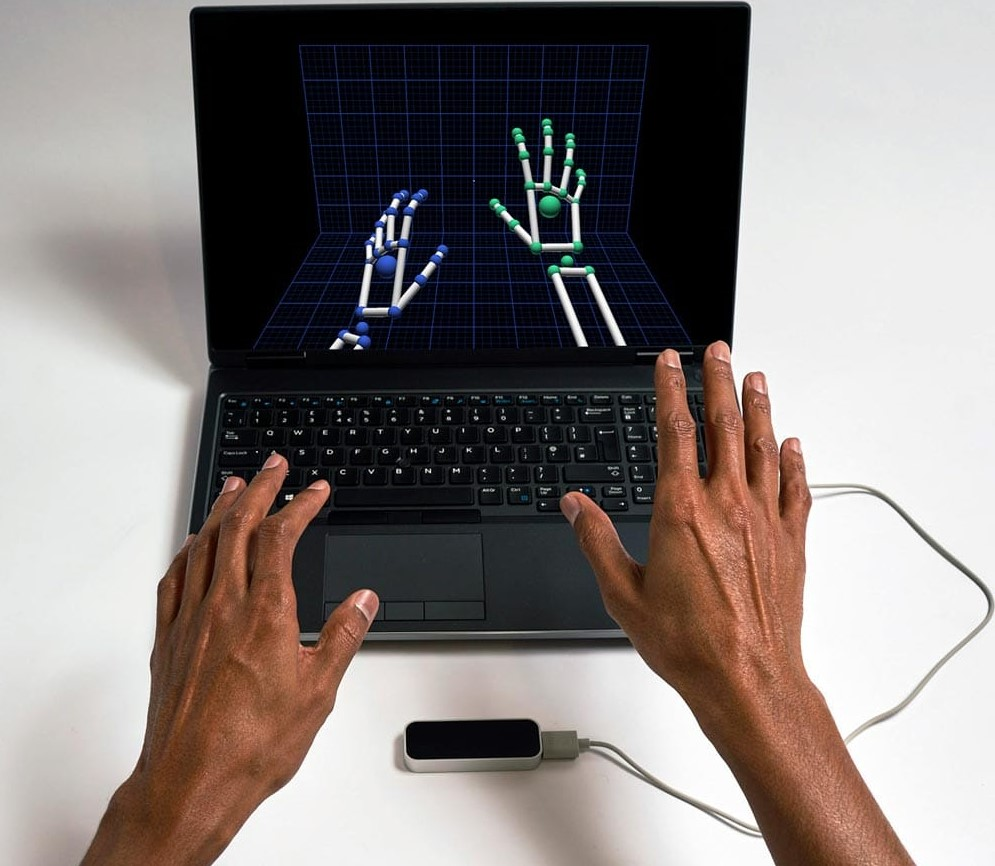
\includegraphics[width=0.5\textwidth]{figures/leapMotion.jpg}
\centering
\caption{Example of the Leap Motion tracking \cite{LEAPROD}}
\label{fig:exampleLeap}
\end{figure}

In order to connect the existing Anonymous Panda prototype with the hand tracking part, it was necessary to use the official UE4 plugin, the Ultraleap Hand Tracking Plugin \cite{ULT}. This plugin allows Unreal developers to make use of the data obtained by incorporating Ultraleap's hand tracking data into their projects. It was designed with the intention of developing and implementing hand tracking in Extended Reality (XR) projects \cite{XR}, but with the right adjustments, it was possible to adapt its use to other types of projects \cite{ULTG}.

As previously stated, the Leap Motion Controller tracks hands and fingers with minimal latency and great precision, reporting position, velocity, and orientation. This controller is suitable for use with a VR headset or on a tabletop. The Leap motion Controller system, which operates as a service or daemon, analyzes the images produced by its hardware and delivers the processed data to the project to combine Ultraleap's hand tracking data. The received data is then converted to the Unreal coordinate system by the Unreal plugin attached to the stated service \cite{ULTP}. Additionally, because the UE employs a left-handed convention for its coordinate system and centimeters as the default unit while the Leap Motion uses a right-handed convention and millimeters as the default unit, the plugin automatically converts the tracking data to utilize a left-handed coordinate system and scales distance values to centimeters \cite{ULTP}. The Unreal coordinate system is shown in Figure \ref{fig:unrealAxes} in relation to the Leap Motion device in Head Mounted Display (HMD) mode.

\begin{figure}[!htb]
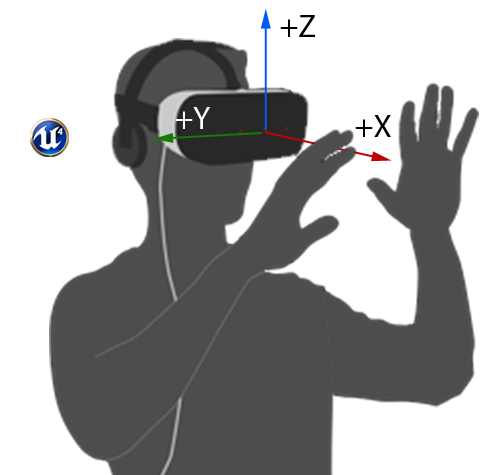
\includegraphics[width=0.4\textwidth]{figures/unrealAxes.png}
\centering
\caption{Relationship of the Leap Motion device in HMD mode to the Unreal coordinate system \cite{ULTP}}
\label{fig:unrealAxes}
\end{figure}

\begin{figure}[!htb]
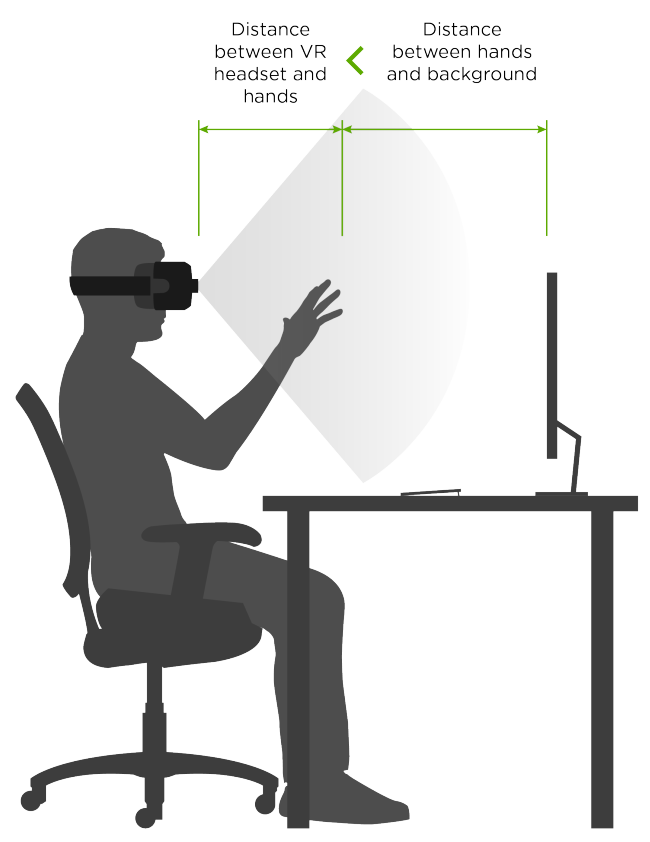
\includegraphics[width=0.4\textwidth]{figures/HMDistance.png}
\centering
\caption{In HMD mode, the sensor should be closer to the hands than the hands should be to any background objects or walls \cite{ULTP}}
\label{fig:HMDistance}
\end{figure}

When the Leap Motion Controller has an excellent, high-contrast view of an object's outline, it detects and tracks it using infrared light and optical sensors. These sensors have a $150^\circ$ field of view and their effective range extends from approximately 3 to 60 centimetres (Figure \ref{fig:HMDistance}). Finally, to handle complicated tracking conditions, the Leap Motion software integrates sensor data with an internal model of the human hand \cite{ULTP}.

\subsubsection{The Hand Tracking Panda}
Because it is a useful, compact device that does not obstruct the face tracking component, we think the Leap Motion Controller is the ideal choice for this work. Therefore, in order to have the best performance in hand tracking, we chose to use the Leap Motion Controller in HMD mode because the Ultraleap Hand Tracking Plugin rotates the 3D hands to keep the correct orientation to the Unreal world when this mode is active \cite{ULTP}. In contrast with the Desktop Mounted Display (DMD) mode (Figure \ref{fig:DMD}), we can see that hand orientation in DMD mode is not ideal for our work since we want to track gestures, which are primarily vertical and happen while individuals are communicating with one another. This concern could be resolved by rotating the data gathered by the Leap Motion Controller before it is applied in the hands of the metahuman, however doing so would cause the prototype to perform slightly slower. We also decided to position the Leap Motion on the chest using a shirt clip made by a 3D printer, as shown in Figure \ref{fig:CMDvsHMD} (b) because using it on a VR support would obstruct the face tracking functionality (imagine having a VR headset as Figure \ref{fig:CMDvsHMD} (a) and wanting the metahuman to blink its right eye).

\begin{table}[!htb]
    \begin{minipage}{\linewidth}
        \centering
        \begin{subfigure}{0.6\textwidth}
            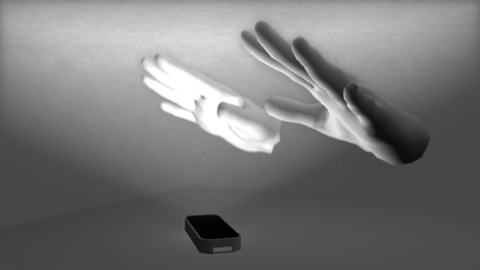
\includegraphics[width=\linewidth]{figures/LeapView.jpg}
            \centering
        \end{subfigure}
        \captionof{figure}{View of hands in DMD mode \cite{ULTP}}
        \label{fig:DMD}
    \end{minipage}
    \begin{minipage}{\linewidth}
        \centering
        \begin{subfigure}{0.4\textwidth}
            \centering
            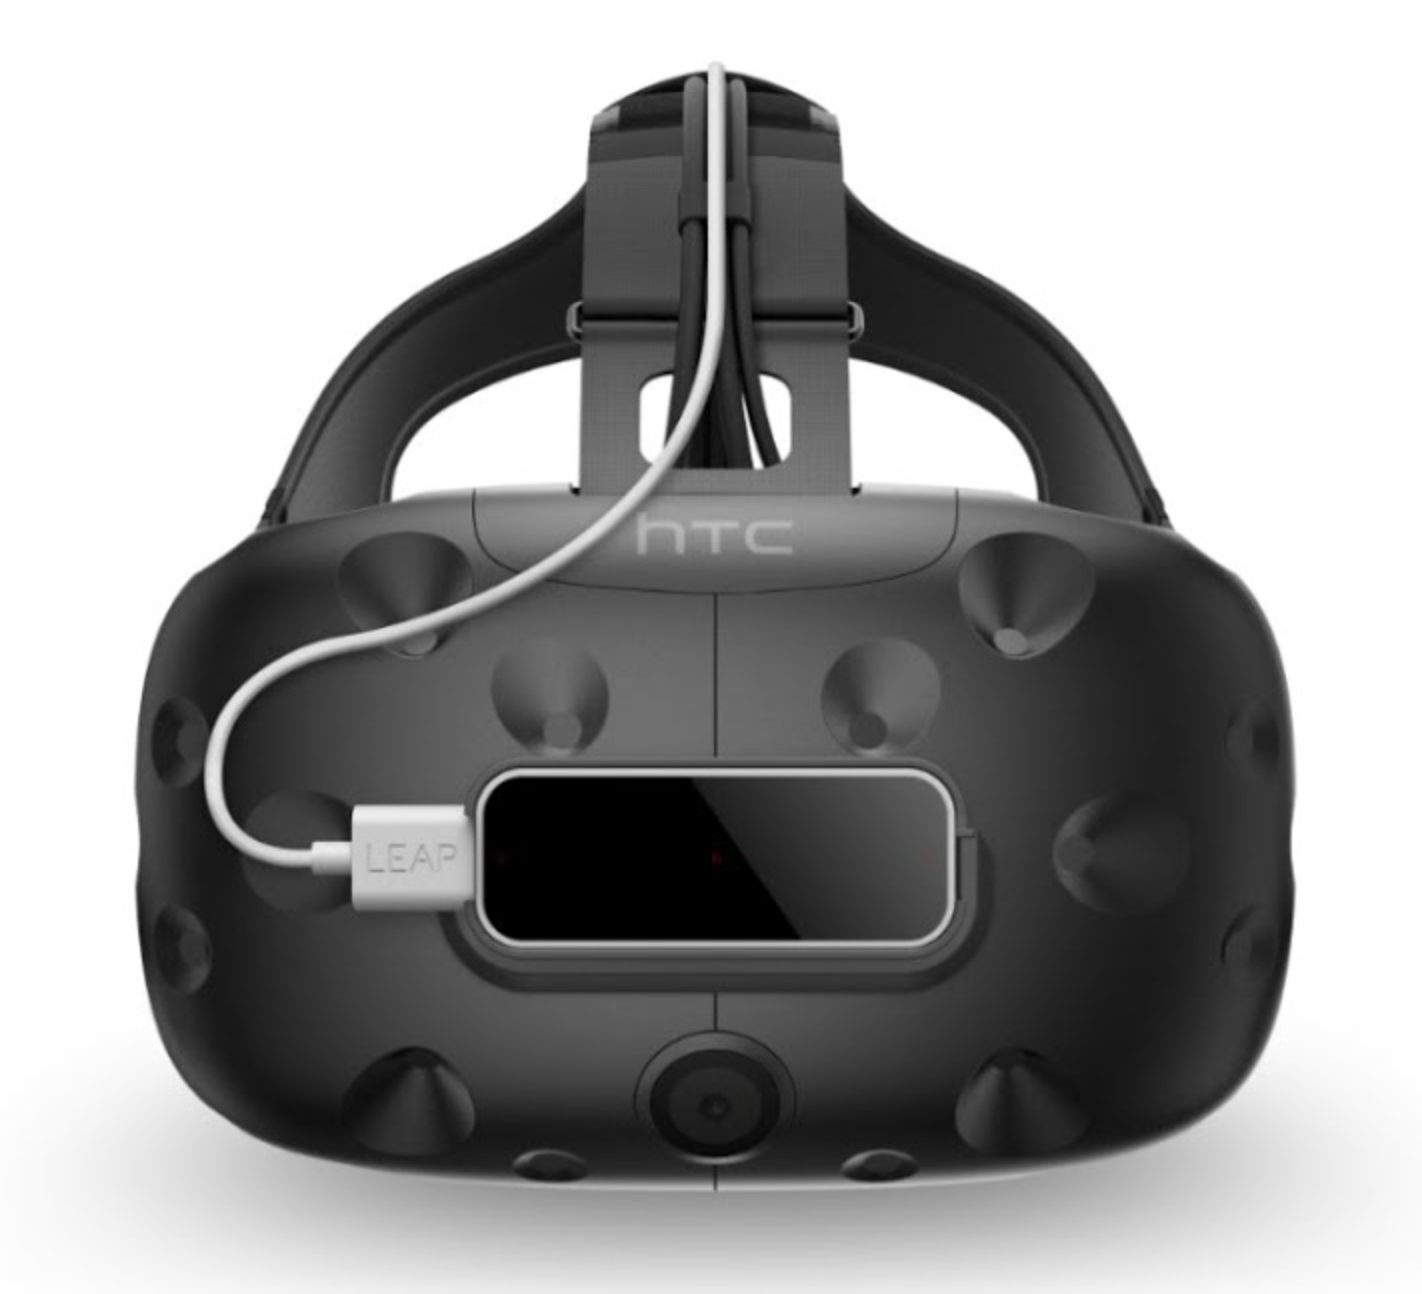
\includegraphics[width=\linewidth]{figures/VRsupport.png}
            \caption{Head (VR support) \cite{LEAPVR}}
        \end{subfigure}
        \begin{subfigure}{0.4\textwidth}
            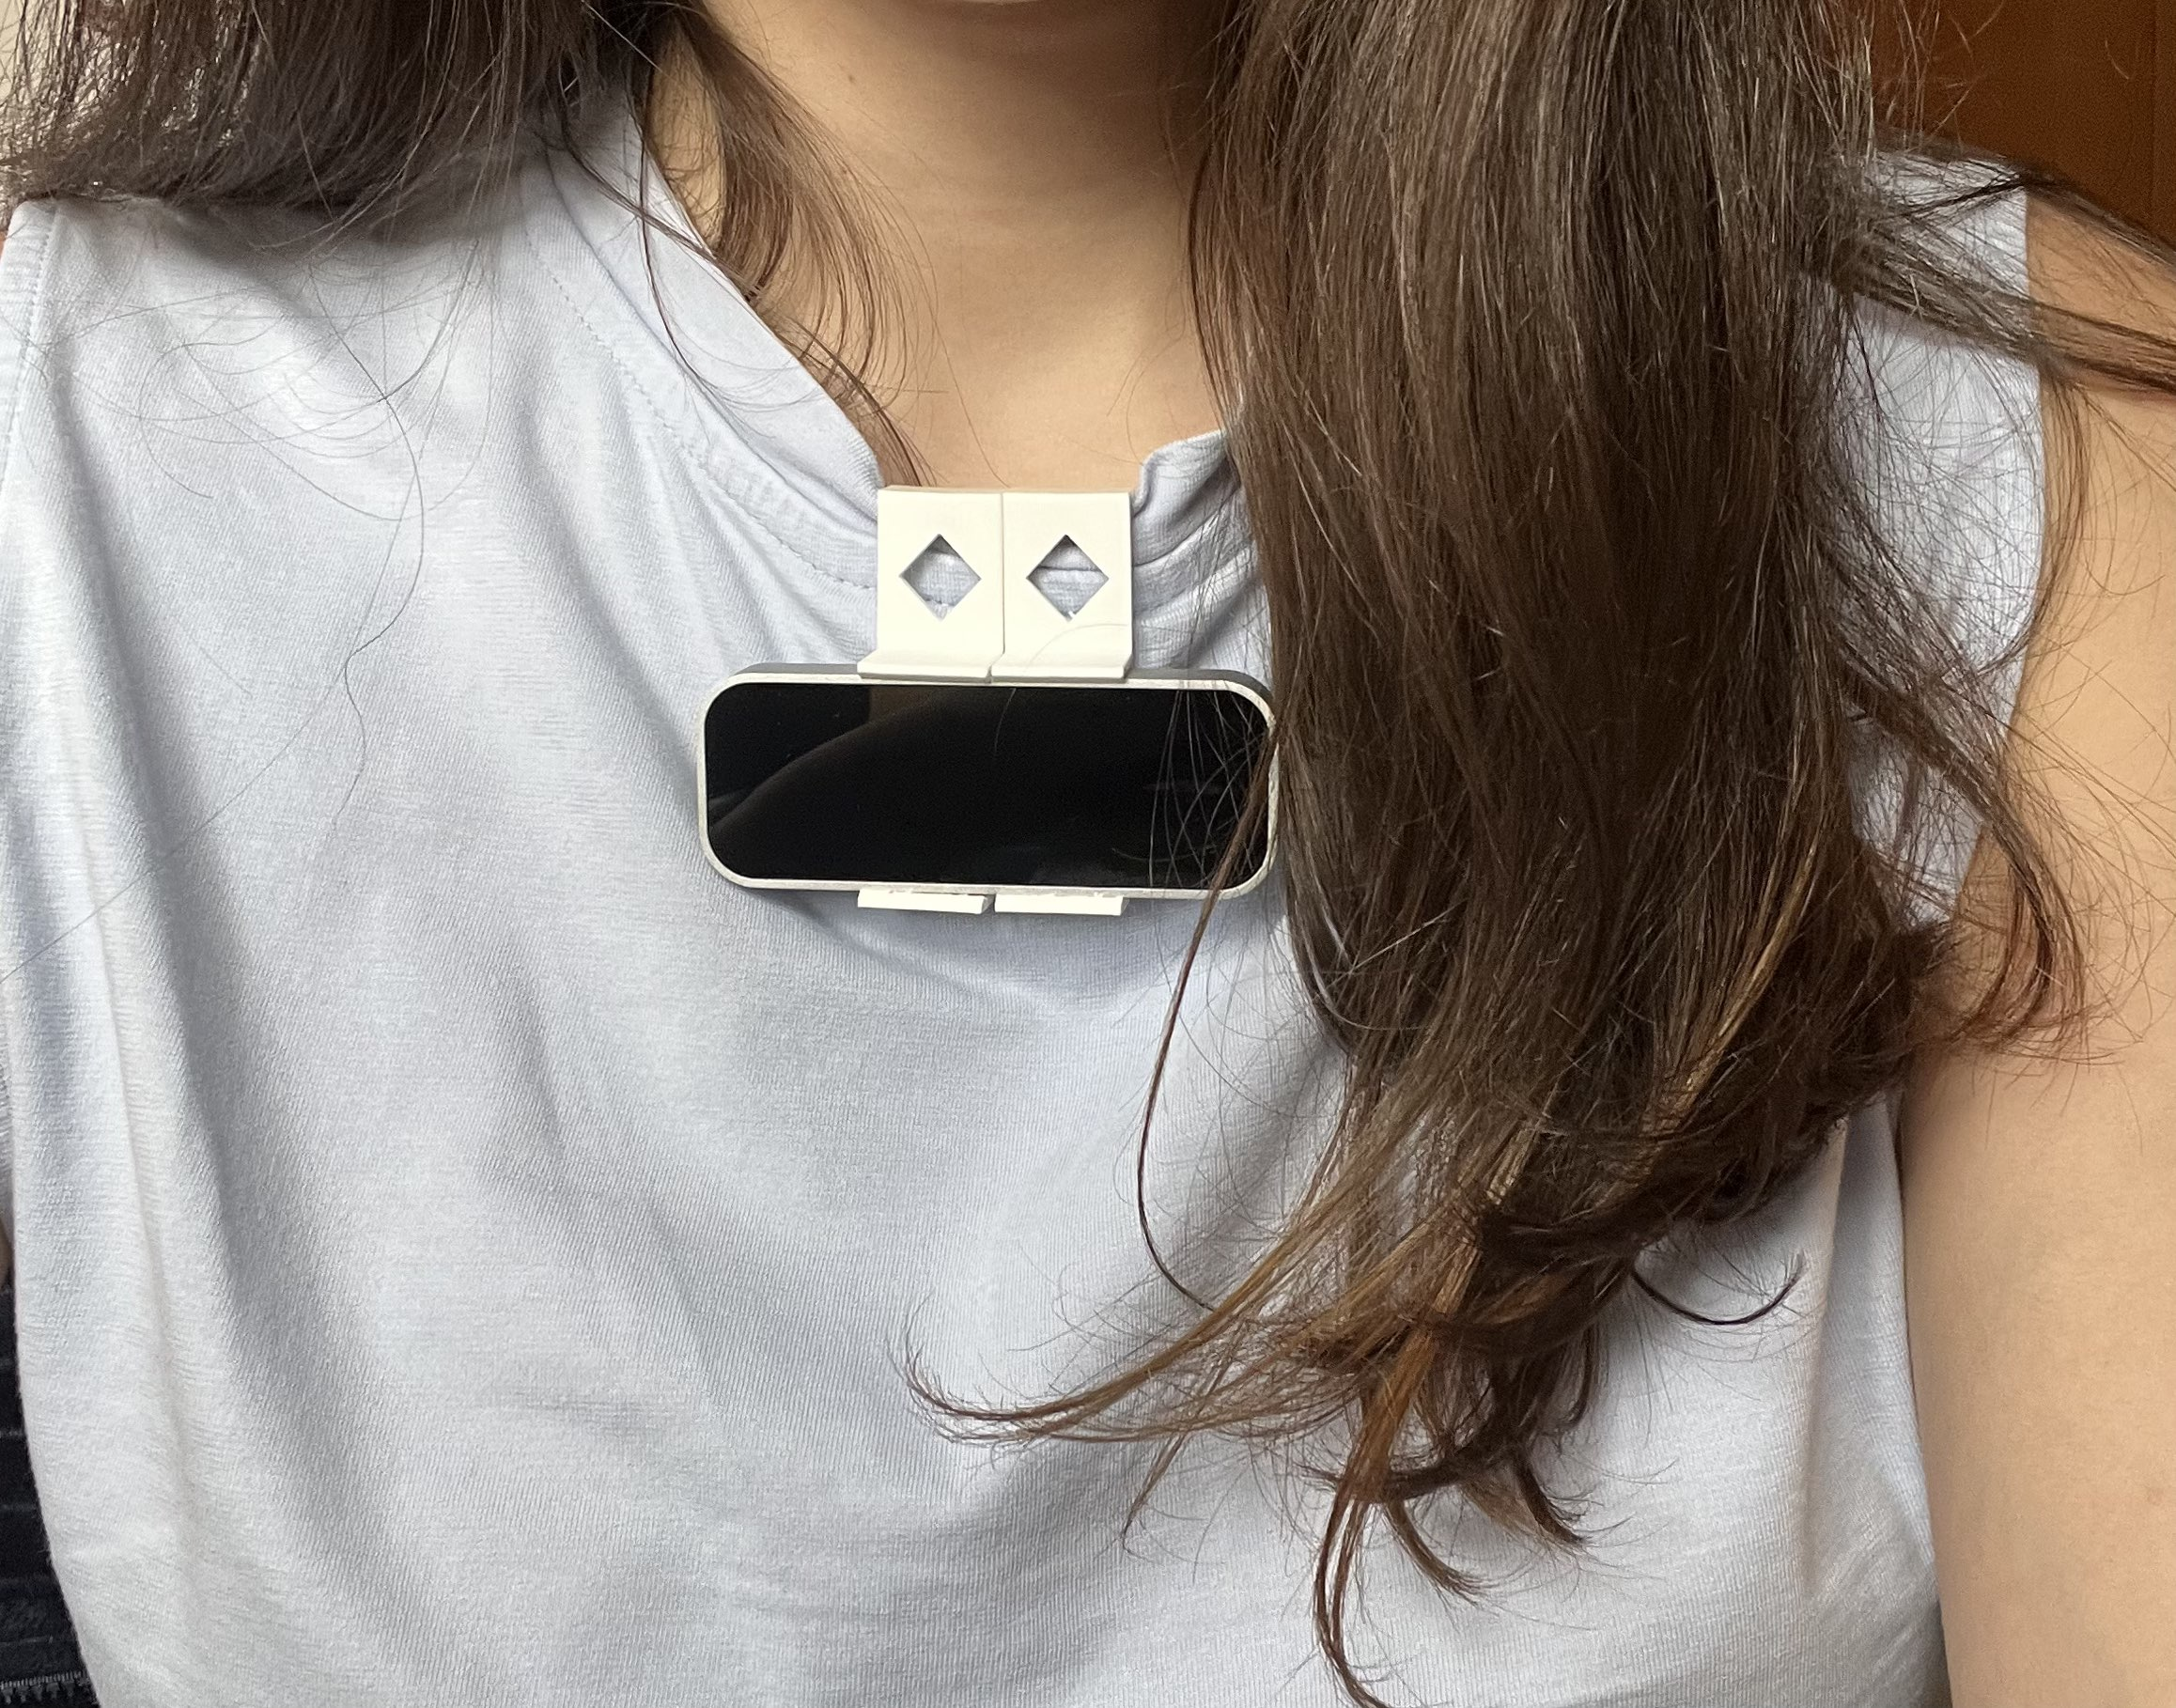
\includegraphics[width=\linewidth]{figures/CMD.jpg}
            \centering
            \caption{Chest}
        \end{subfigure}
        \captionof{figure}{Head vs. Chest Mounted Mode}
        \label{fig:CMDvsHMD}
	\end{minipage}
\end{table}

The official Ultraleap Tracking Plugin for Unreal Engine 4 utilizes pre-made blueprints to add hand tracking to a scene and play it in the editor. However, depending on the project, it may take a more customized approach using C\texttt{+}\texttt{+} or blueprints \cite{ULTGIT}. For our project, we attempted to adapt a custom rigging example map from the Ultraleap Plugin, which contained several animation blueprints \cite{LEAPMOD}, to create the new version of the Anonymous Panda prototype, beginning by seeing how each rigging was done and how we could adapt it to our metahumans' bones.

To use the rigging on our metahumans effectively, we had to re-parent the metahuman animation blueprint to "BodyStateAnimInstance". By utilizing the Body State system, we were able to map the tracked data collected by the Leap Motion Controller to the metahumans' skeletal mesh bones (Figure \ref{fig:mappedBones}).

\begin{table}[!htb]
    \begin{minipage}{\linewidth}
        \centering
        \begin{subfigure}{0.49\textwidth}
            \centering
            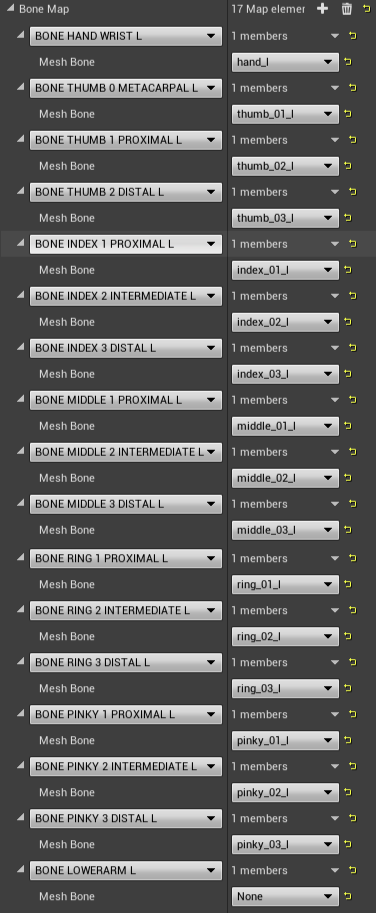
\includegraphics[width=\textwidth]{figures/mappedBones.png}
            \caption{Left Side}
        \end{subfigure}
        \begin{subfigure}{0.49\textwidth}
            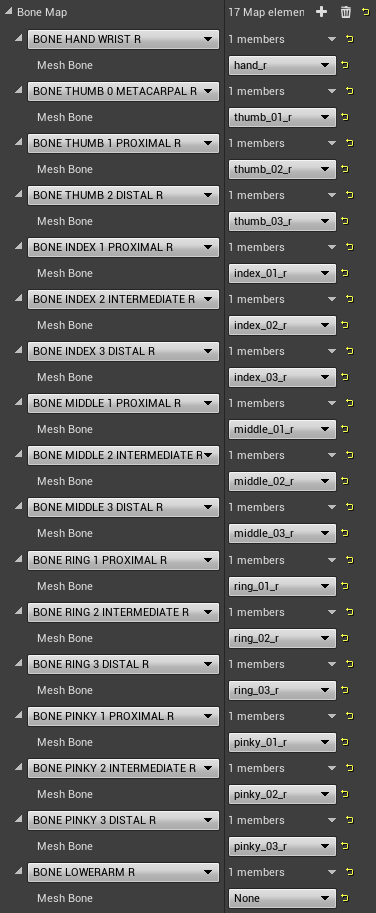
\includegraphics[width=\textwidth]{figures/mappedBonesR.png}
            \centering
            \caption{Right Side}
        \end{subfigure}
        \captionof{figure}{Tracked data mapped to the metahumans' skeletal hands mesh bones}
        \label{fig:mappedBones}
	\end{minipage}
\end{table}

We used the two Mapped Bone Anim Data arrays that were previously seen (Figure \ref{fig:mappedBones}), much like the two-handed example from the custom rigging map, and chose to disable the deformation mesh because the metahuman model does not yet allow deformation (Figure \ref{fig:mappedBoneList}).

\begin{figure}[!htb]
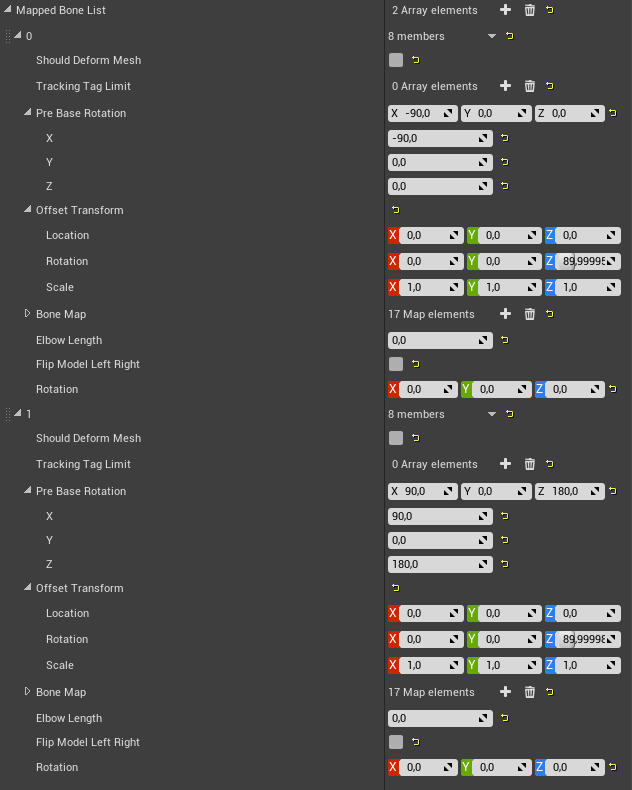
\includegraphics[width=0.8\textwidth]{figures/mappedBoneList.png}
\centering
\caption{Mapped Bone List}
\label{fig:mappedBoneList}
\end{figure}

Since we disabled the deformation mesh, only the rotations were tracked. To move the elbows to their proper positions, we apply an animation node called Forward And Backward Reaching Inverse Kinematics (FABRIK) to each elbow. The FABRIK animation node is an Inverse Kinematics (IK) solver that handles joint rotation from the location of an end-effector rather than directly from the joint rotation.  In practice, we designate an effector point, and the IK solution rotates the joint to be as close to that place as possible \cite{IK}.

The majority of animated skeletons in UE are powered by direct rotational data fed into the character's bones or the Skeletal Mesh. This is known as Forward Kinematics (FK), or the direct application of rotation to joints or bones \cite{IK}. Figure \ref{fig:kinematics} (a) illustrates a diagram of the concept.

Inverse Kinematics, on the other hand, works in the opposite way. Instead of rotating bones, we give the bone chain a target (also known as an end effector) that specifies where the chain's end should aim. The user moves the effector, and the IK solver (the algorithm that drives rotation in an IK system) rotates the bones until the last bone in the chain reaches the target location \cite{IK}. The end effector is shown by the red cross in Figure \ref{fig:kinematics} (b).

\begin{table}[!htb]
    \begin{minipage}{\linewidth}
        \centering
        \begin{subfigure}{0.49\textwidth}
            \centering
            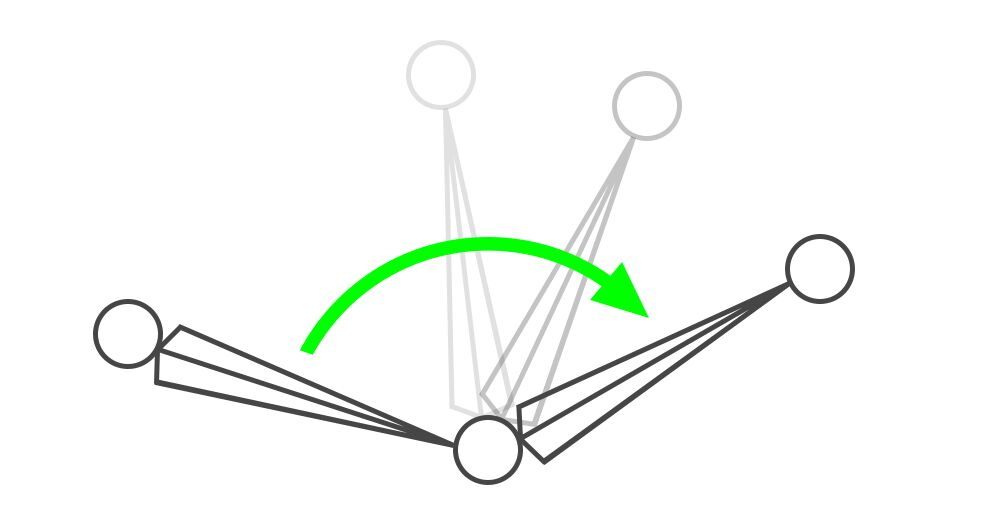
\includegraphics[width=0.8\textwidth]{figures/diagram_FK.png}
            \caption{Forward Kinematics \cite{IK}}
        \end{subfigure}
        \begin{subfigure}{0.49\textwidth}
            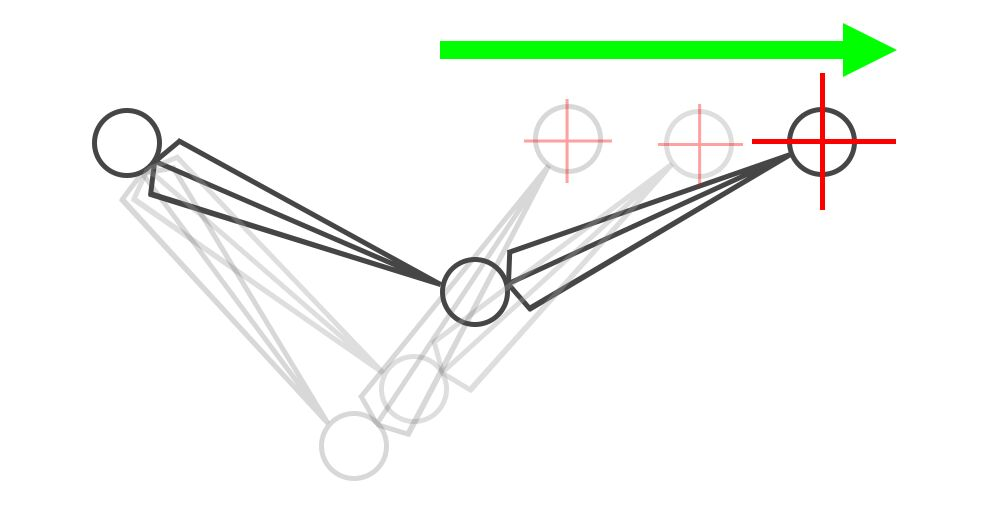
\includegraphics[width=0.8\textwidth]{figures/diagramIK.png}
            \centering
            \caption{Inverse Kinematics \cite{IK}}
        \end{subfigure}
        \captionof{figure}{Diferences between FK and IK}
        \label{fig:kinematics}
	\end{minipage}
\end{table}

Once again, in order to position the shoulders correctly, we had to rotate all of our mapped data by 90 degrees in the "Offset Transform" for Y, as is typical for skeletal meshes and as shown in Figure \ref{fig:mappedBoneList}.

Concerning the prototype's outcome, Figure \ref{fig:BPHandsAndIK} depicts the steps taken from providing the IK with all of the data required for its operation to the metahuman's animation in the blueprint, after gathering data for the hands animation. Finally, Figure \ref{fig:handTrack} and videos \cite{APT1,APT2} illustrate the outcome applied to one of the metahumans used in this study.

\begin{figure}[!htb]
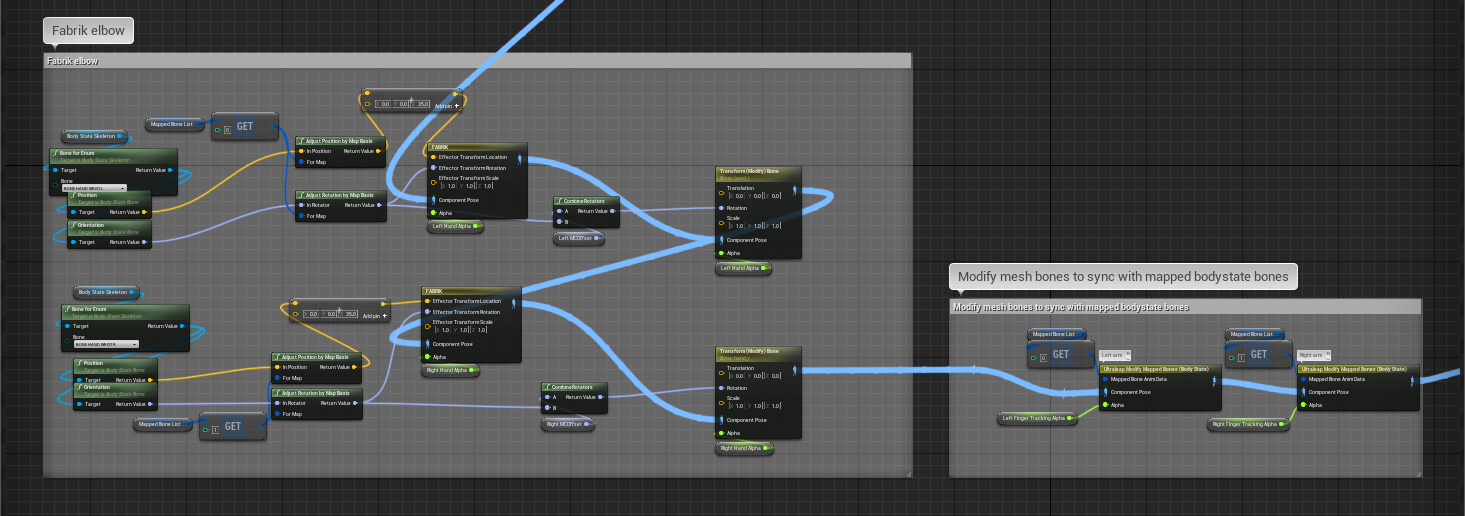
\includegraphics[width=\textwidth]{figures/BPHandsAndIK.png}
\centering
\caption{Part of the blueprint in control of animating metahuman hands using data collected by leap motion}
\label{fig:BPHandsAndIK}
\end{figure}

\begin{figure}[!htb]
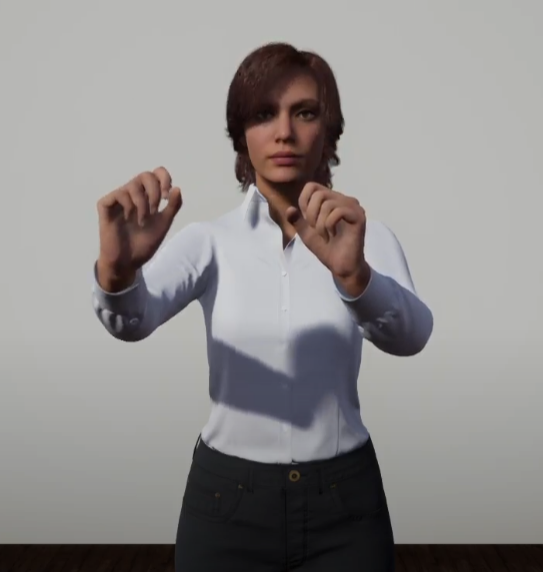
\includegraphics[width=0.5\textwidth]{figures/final.png}
\centering
\caption{The hand tracking's final outcome}
\label{fig:handTrack}
\end{figure}

\paragraph{Challenges}
The exploration of the ultraleap plugin was one of the first challenges encountered during the development of this version of the prototype. Despite being documented, the examples provided were difficult to replicate due to the limited amount of online content that could help with this issue. We tried using github issues to ask for help since the solution was still far from being found but were unsuccessful. We eventually addressed the problem by downgrading the plugin version to version 4.2.0. 

After we were able to successfully reproduce the plugin demonstrations, we made the decision to investigate hand tracking using the rigging method. Following the example of the custom rigging map, we adapted some of its content to our animation blueprints, but we were unable to achieve the same effect as the rigging example. Our initial attempt is shown in Figure \ref{fig:initialSteps} (a), which only shows the left arm, and Figure \ref{fig:initialSteps} (b), which shows both arms. The shoulders and hands in both figures have a significant deformation, but they were still capable of movement.

\begin{table}[!htb]
    \begin{minipage}{\linewidth}
        \centering
        \begin{subfigure}{0.49\textwidth}
            \centering
            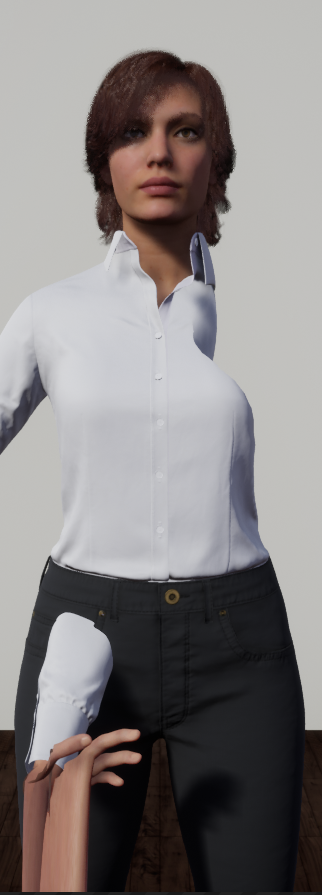
\includegraphics[width=0.5\textwidth]{figures/issue.png}
            \caption{Hand and Shoulder deformation}
        \end{subfigure}
        \begin{subfigure}{0.49\textwidth}
            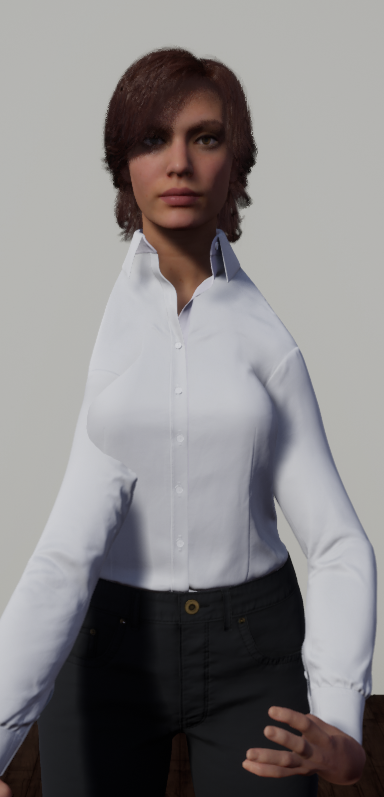
\includegraphics[width=0.67\textwidth]{figures/FirstInteraction.png}
            \centering
            \caption{Hands and Shoulders deformations}
        \end{subfigure}
        \captionof{figure}{Initial Hand Tracking Steps}
        \label{fig:initialSteps}
	\end{minipage}
\end{table}

The leap motion controller broke while we were trying to solve this issue, and we had to wait 3 weeks for a replacement. Since this device was absolutely necessary for the project, we used these three weeks to search for solutions online, in the plugin's documentation, and in github issues. In the end, we discovered a video on YouTube featuring a metahuman who could move his arms using the hand tracking data from leap motion \cite{TVL}. After contacting the person who uploaded the video, we were able to get them to provide some advice and tips about how hand tracking should be used properly in Unreal Engine. We made an effort to stick to the advice provided, but we were unable to achieve the desired outcome. The result, in which the arms were infinitely stretched, is shown in Figure \ref{fig:armsStretching}.

\begin{figure}[!htb]
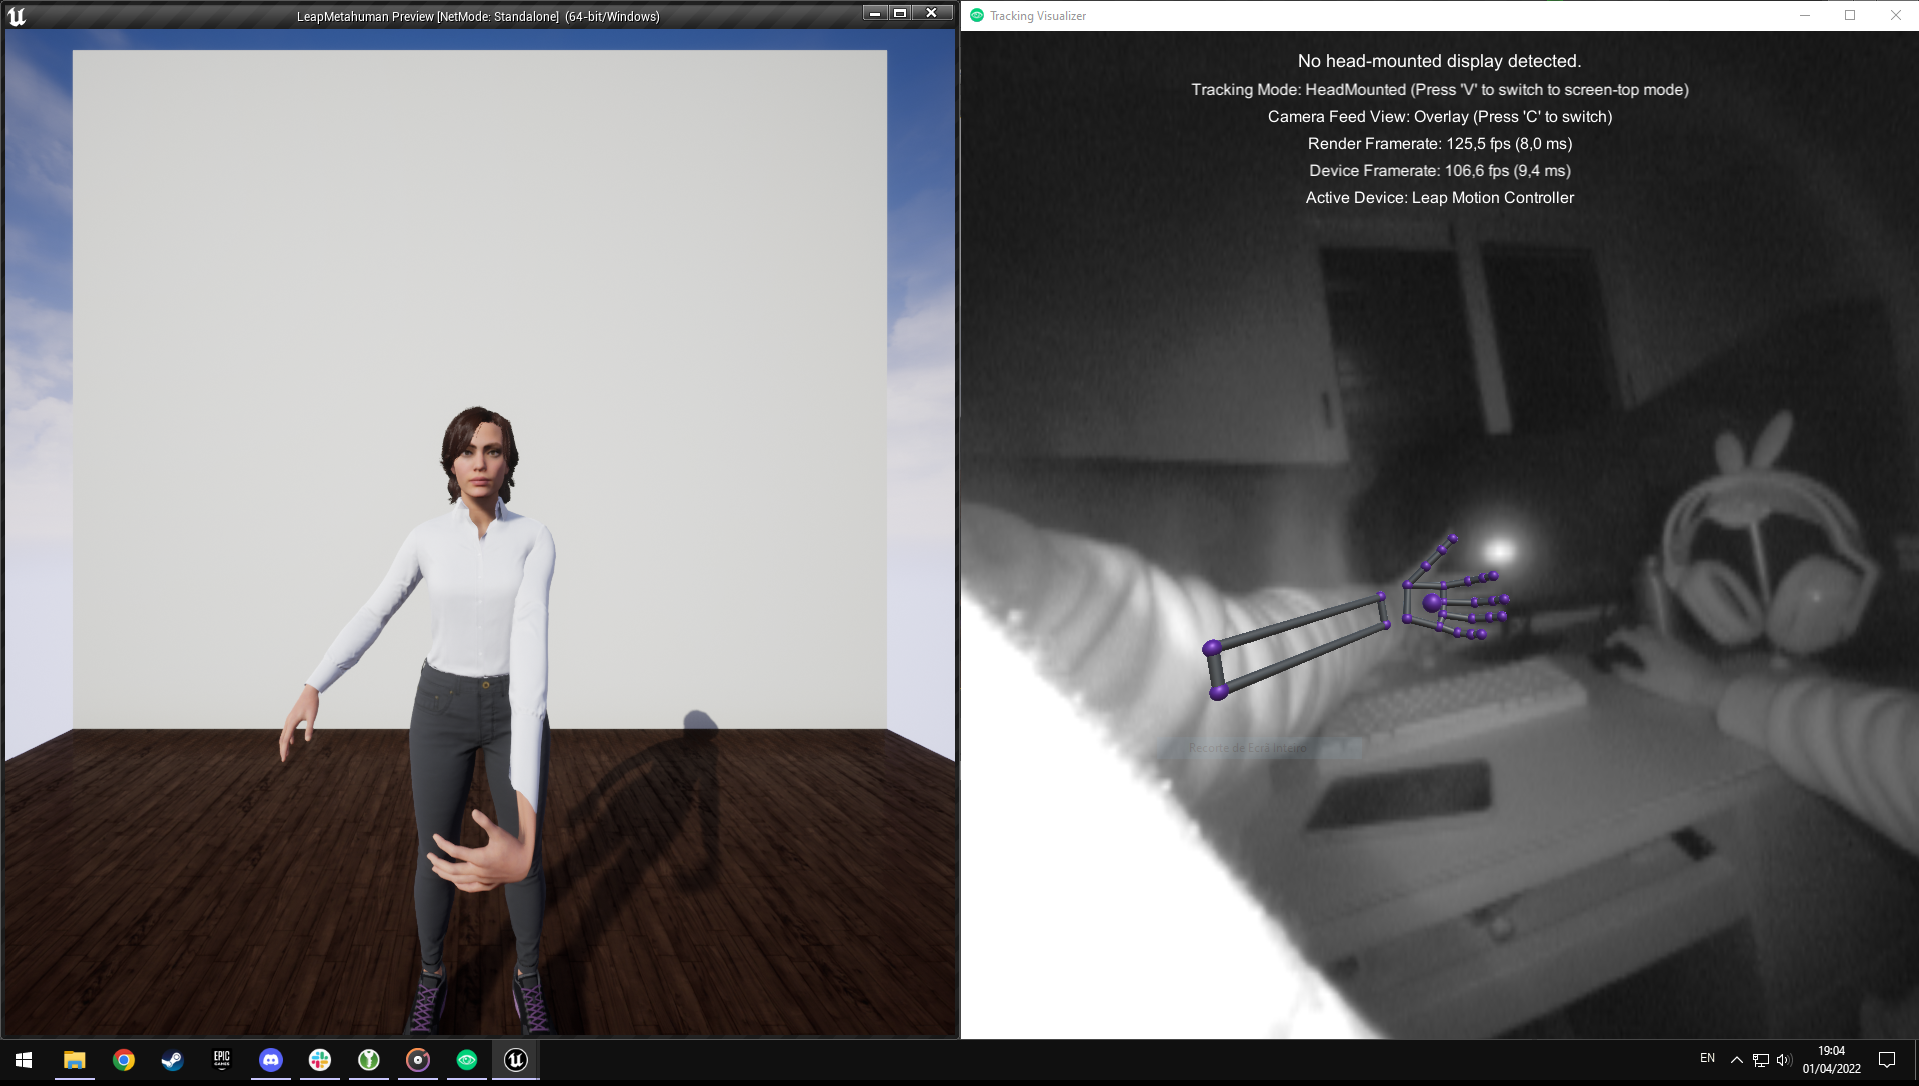
\includegraphics[width=\textwidth]{figures/handStretching.png}
\centering
\caption{Left arm stretching infinitely}
\label{fig:armsStretching}
\end{figure}

We got in touch with the person from the video again, and he gave us additional advice on how to handle this. The result can be observed in Figure \ref{fig:closeOutcome} and we can notice that the outcame is getting closer to what we wanted (Figure \ref{fig:handTrack}). Still, in order to achieve a more realistic effect, we must elevate our metahumans' hands to waist level.

\begin{figure}[!htb]
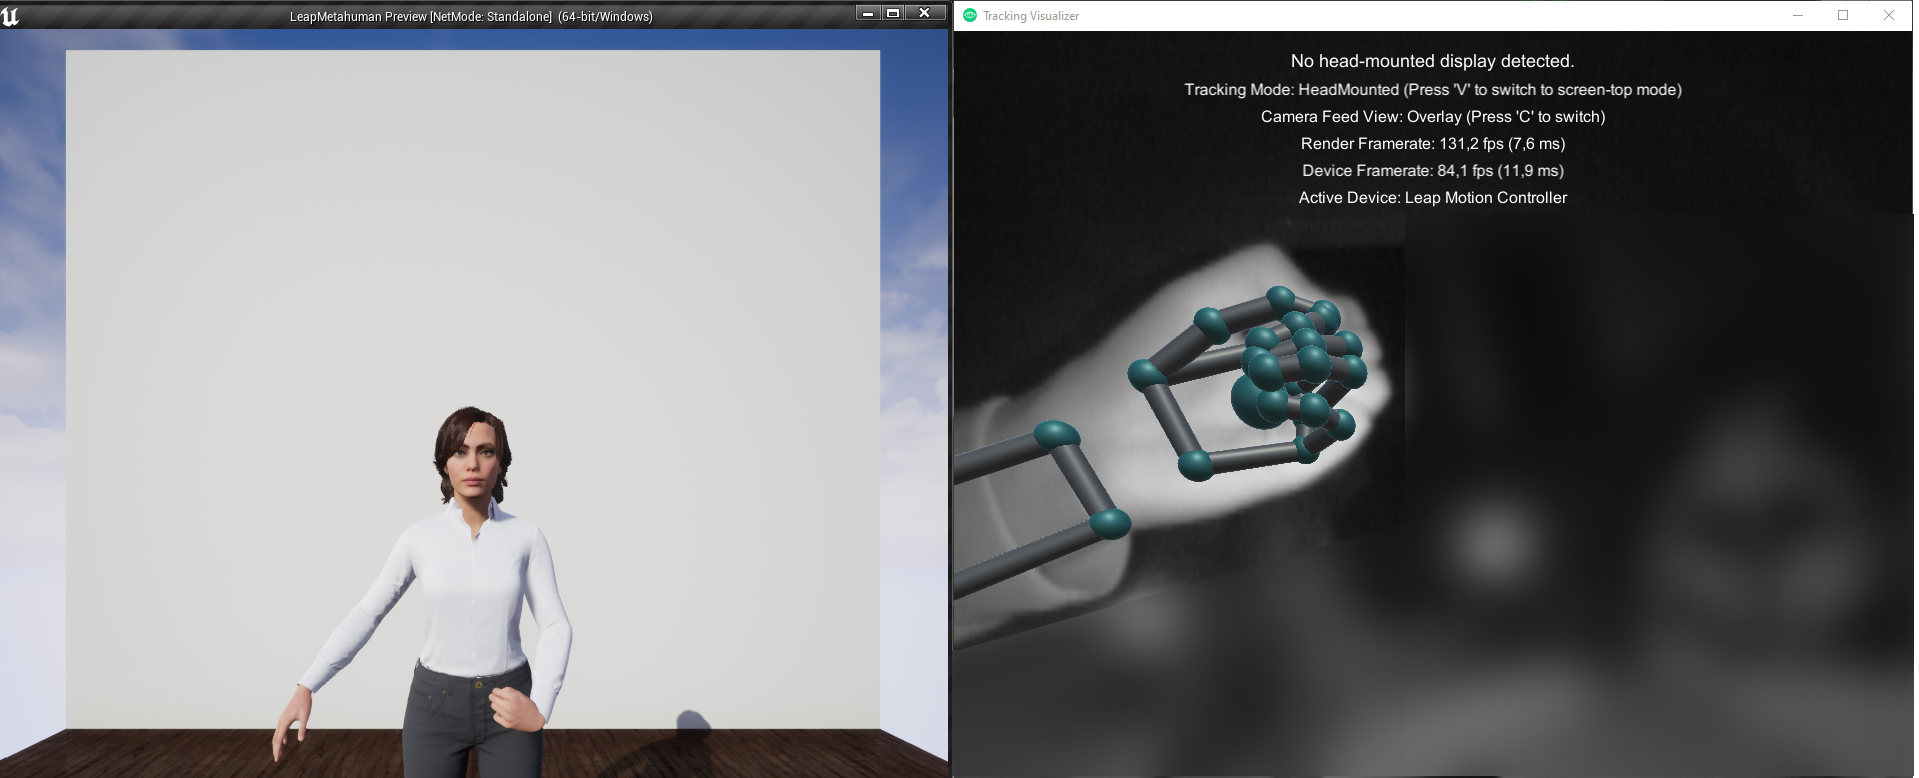
\includegraphics[width=\textwidth]{figures/handMinPosition.png}
\centering
\caption{One step closer to the final outcome}
\label{fig:closeOutcome}
\end{figure}

To offset the metahumans' hands and raise them to waist height, we followed the advice of the individual who uploaded the YouTube video and added a positive constant on the Y-axis to the "Effector Transform Location" vector before the IK solver performed its magic. Although the output was closer to what was intended, the fingers stopped functioning normally (Figure \ref{fig:fingersIssue} and video \cite{APT3}).

\begin{figure}[!htb]
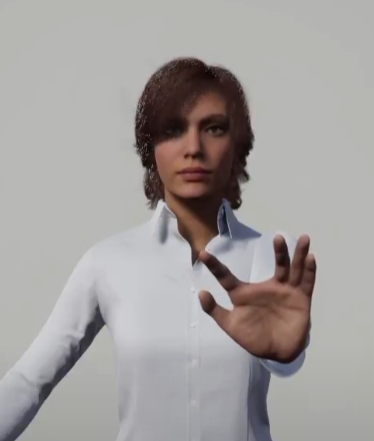
\includegraphics[width=0.5\textwidth]{figures/otherIssue.png}
\centering
\caption{Issues with the fingers as the outcome neared}
\label{fig:fingersIssue}
\end{figure}

While trying to figure out how to get the fingers to work properly again, we received a new tip to not map the metacarpal bones of the fingers, which solved our problem. However, the arms started to stretch out indefinitely once more (Figure \ref{fig:armsStretching}). To solve this issue, we noticed that mapping the lower arm to none solved the problem, and thus we obtained our final result (Figure \ref{fig:handTrack}).

\paragraph{Limitations}
As was already noted, many studies think that hand gestures, along with facial expressions and spoken words, are important in expressing our emotions. In order to achieve our goal of deeper emotional recognition, including hand tracking to the existing prototype was a crucial step. Because hands are the most crucial nonverbal clues for identifying particular states in others, after facial expressions and body position \cite{WAX97, REI22}.

There are a number of ways to accomplish hand tracking, such as with virtual reality equipment or gloves, but we felt that the Leap Motion Controller was the ideal choice for this work because it is a useful and compact device that does not interfere with the face recognition component. This device, however, has significant limitations. There is a reliance on the usage of the USB cable for leap motion and unreal communication, and because it is an old device, acquiring it may be difficult. Additionally, infrared sensors may not function properly in bright environments, and turning on the HMD mode requires the Ultraleap Visualizer program rather than the blueprint configuration because doing so interferes with the hand tracking data.

Last but not least, a 3D-printed dependency of two shirt clips is shown in Figure \ref{fig:CMDvsHMD} (b). In the beginning, only one shirt clip was required, however throughout the prototype tests, instability and imprecise hand tracking capture were detected. Although the two clips are currently functional, a more stable and user-friendly solution would be preferable.

\subsubsection{Anonymous Panda User Interface}
There was some feedback from friends and family on the prototype interface during several project demonstrations. Much of this feedback was connected to the lack of other metahumans, which were present but the opportunity to switch between them was not easily identified, and users were always forced to choose between the initial two metahumans since they were unaware of this option.
In response to these critiques, we made an effort to develop a new user interface that was simpler to use and made all of the prototype's metahumans available at the time of user selection (Figure \ref{fig:newUI}). Since the prior study did not allow us to test the user interface with actual users, we were unable to identify this issue which could have been addressed earlier. We anticipate to get further feedback on this problem in the upcoming study by testing the User Interface (UI) with actual users and, if necessary, changing it.

\begin{figure}[!htb]
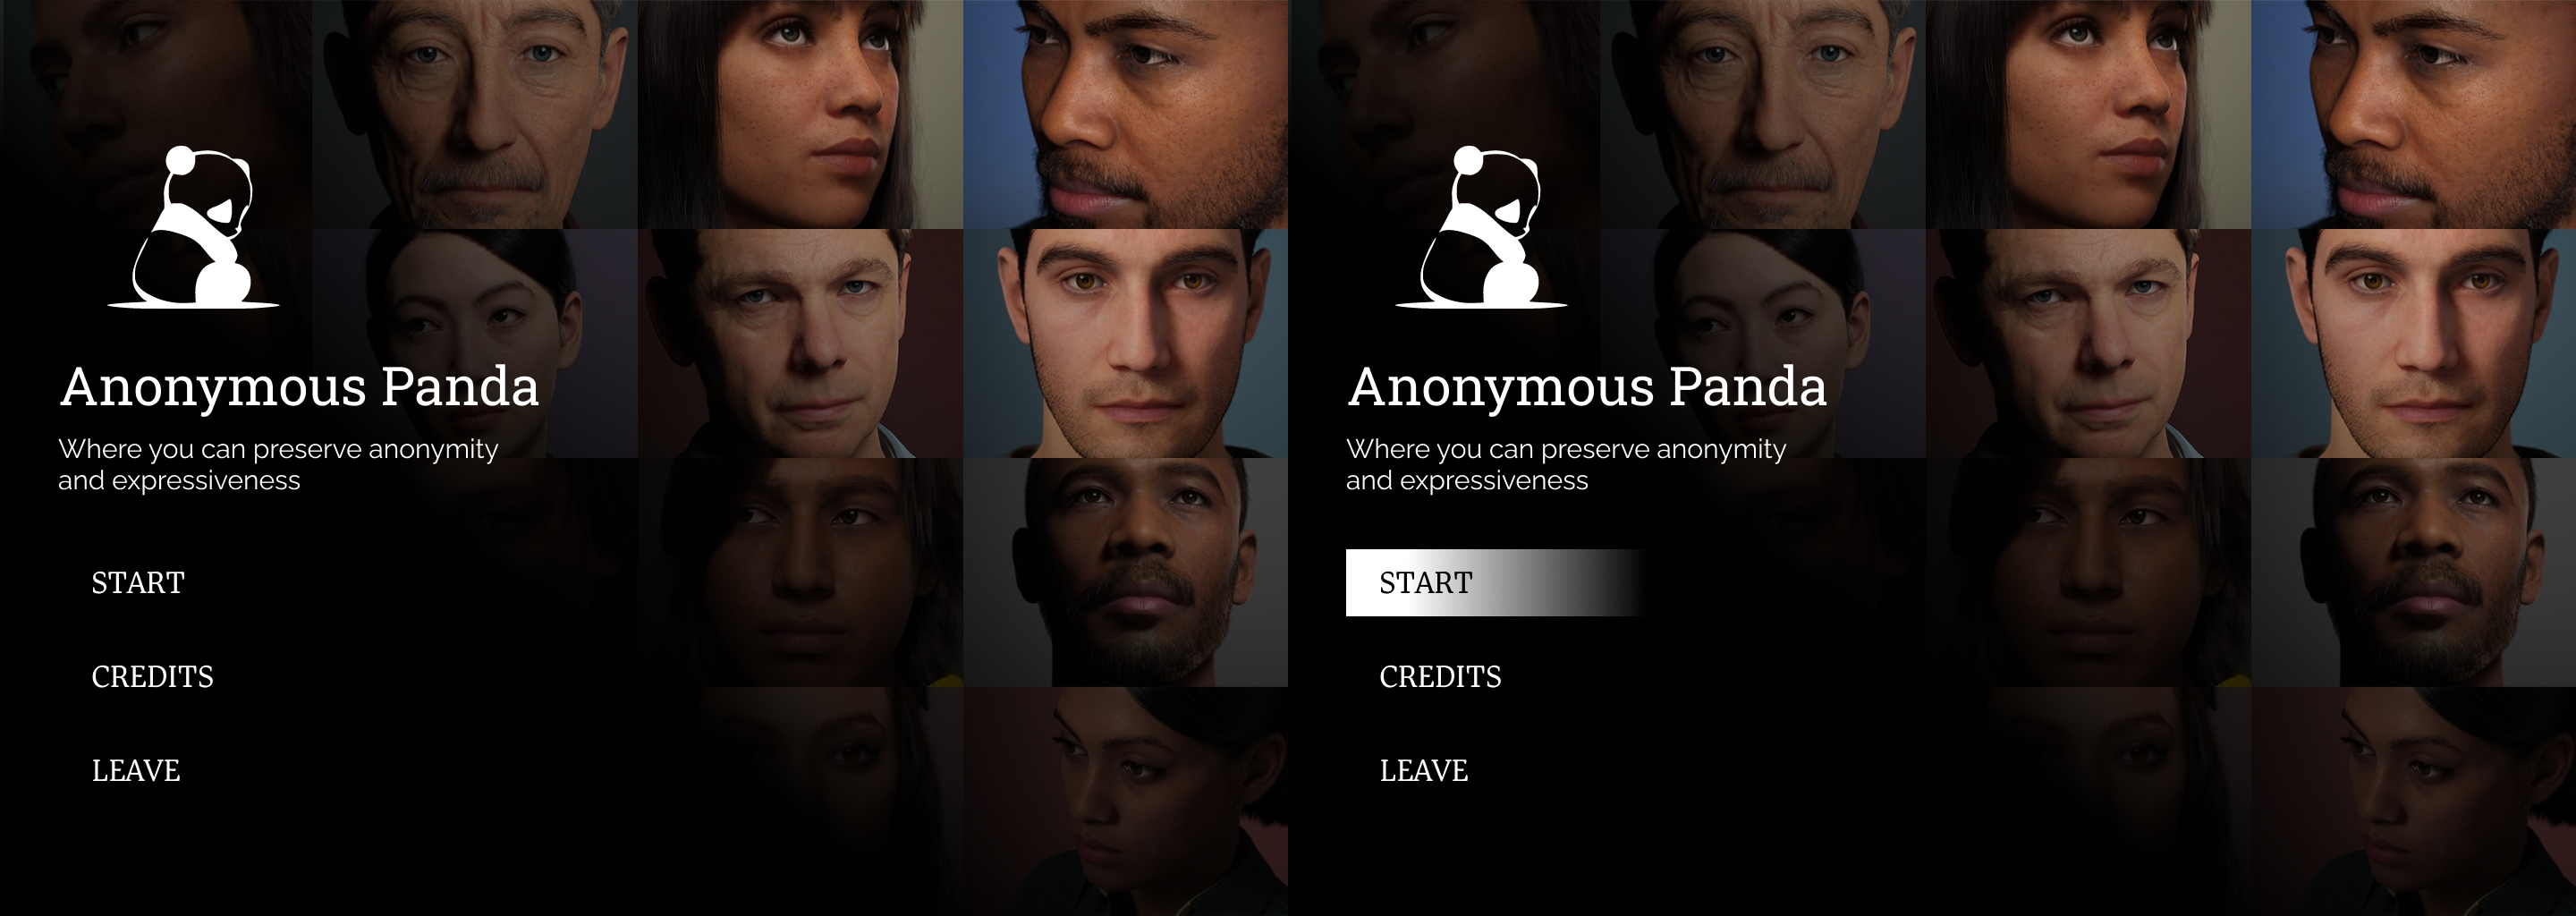
\includegraphics[width=\textwidth]{figures/startMenu.png}
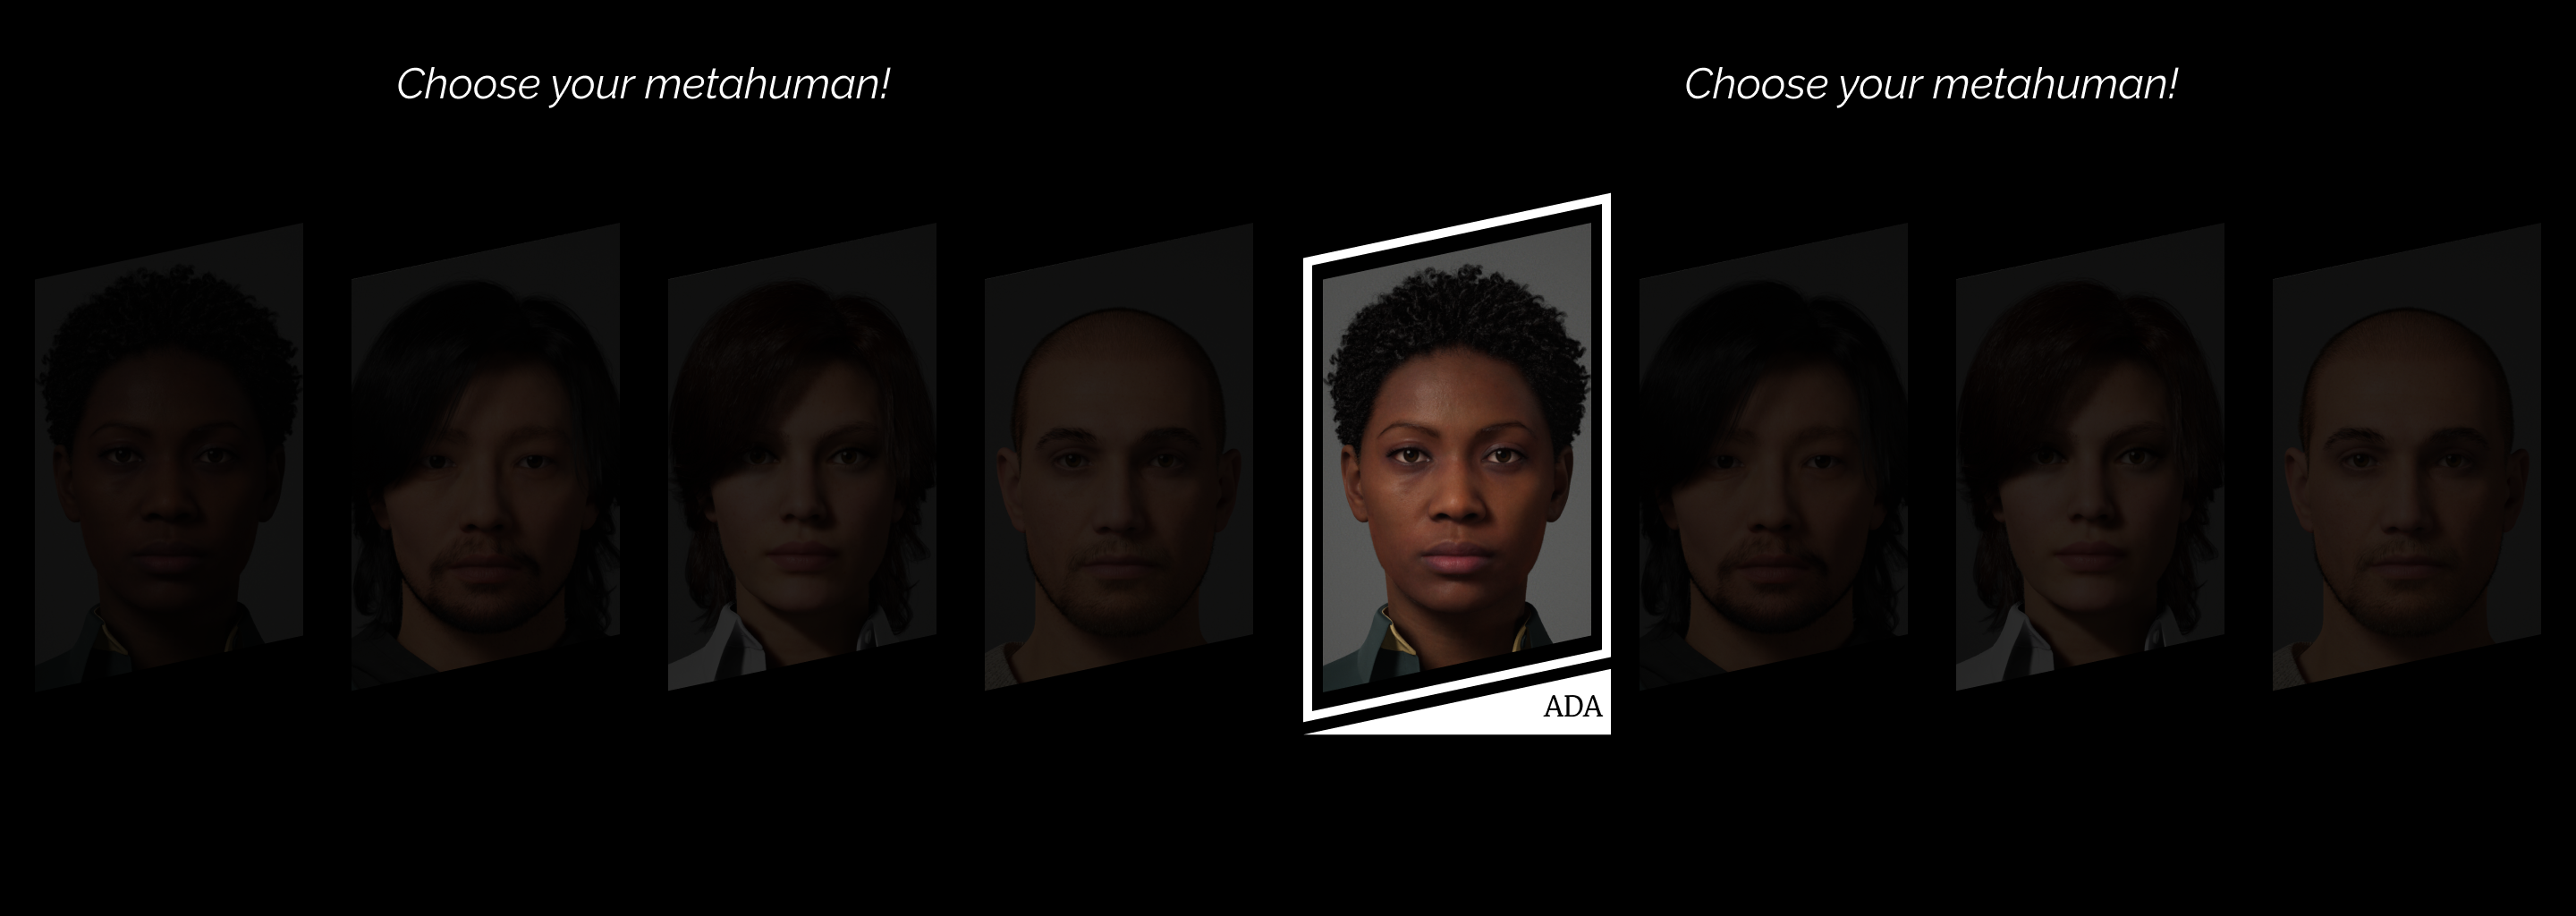
\includegraphics[width=\textwidth]{figures/metahumanMenu.png}
\centering
\caption{New Anonymous Panda UI}
\label{fig:newUI}
\end{figure}

\subsection{Methodology}
The purpose of this study is to put to the test an extended Technology Acceptance Model (TAM) created to study user acceptance of our work, the Anonymous Panda. Furthermore, we want to see if virtual avatars can help promote interactants' verbal self-disclosure or not (\textbf{RQ\textsubscript{2}}).

Based on two user perceptions: perceived utility and perceived ease of use, the TAM estimates user intention to utilize a particular technology. Perceived usefulness is defined as "the amount to which a person believes that using a certain system will improve his or her job performance" \cite{DAV89}. In contrast, perceived ease of use is defined as "the degree to which a person believes that using a certain technology would be devoid of effort" \cite{DAV89}.

The Technology Acceptance Model is a practical model that can be applied in a lot of situations, and it has been refined via several research to accommodate various technologies, situations, and users. TAM adaptations have been proposed for features from similar models (e.g., subjective norm, perceived behavioral control), new belief factors (e.g., triability, content richness), and external variables (e.g., demographic characteristics, computer self-efficacy) \cite{CAM20}. External variables can act as predictors or moderators of perceived usefulness and usability. By including new variables, these extensions try to improve the TAM's capacity to predict outcomes for specific technologies, situations, and users \cite{CAM20}.

Several investigations using the TAM to analyze a person's intention to utilize specific technologies have shown that the TAM can be beneficial in a broad range of situations \cite{CAM20}. Furthermore, they discovered that perceived utility and perceived simplicity of use predicted use intention. And finally, discovered a significant relationship between perceived ease of use and perceived usefulness. However, to the best of our knowledge, little research has been conducted on the relationship between Perceived Anonymity (PA) and Online Public Disclosure (OPD), two important variables for our research.

To assess the feasibility of the previously described approach and test users' acceptance of our application, as well as users' OPD, we conducted a controlled prototype testing in order to assess if the Anonymous Panda had an effect on participants' perceived anonymity (PA), online public disclosure (OPD), perceived usefulness (PU), and perceived ease of use (PEU), which can help us demonstrate users' acceptance.

\subsubsection{Participants}
Participants were required to be at least 18 years old and a member of the Interactive Technologies Institute. They were personally invited to partake in the research and were given a general overview of the study's topic. Our final sample consists of 20 individuals (11 males, 9 females), aged between 18 and 46 (\textit{M}=28.75, \textit{SD}=6).

Those who agreed to participate (\textit{N}=20) were first given an informed consent form. Participants were asked to fill out basic demographic questions as well as a self-assessment questionnaire to determine their baseline levels of online public disclosure for this experiment. They were then taken to a room for at least 2 minutes to test our prototype before being asked some follow-up questions.

\subsubsection{Procedure}
To recruit participants, we personally announced the start of our study to the entire Interactive Technologies Institute population. Those who were interested in our work and agreed to participate in the study (\textit{N}=20) were first given an informed consent form (see Appendix \ref{appendix:consentDemographic}) and were fully informed about the study's broad and general topic.

Participants were asked to fill out basic demographic questions (see Appendix \ref{appendix:consentDemographic}) as well as some questions about their OPD, as proposed by \cite{YUN06}. They were then led to a room with a setup (see Figure \ref{fig:setup}) where they could test our prototype for a short period of time (see Figure \ref{fig:userTesting}). Participants were not assigned any specific tasks; instead, they were simply asked to interact with the prototype and test the different tracking sensors.

\begin{figure}[!htb]
\centering
    \begin{minipage}{0.49\textwidth}
        \centering
        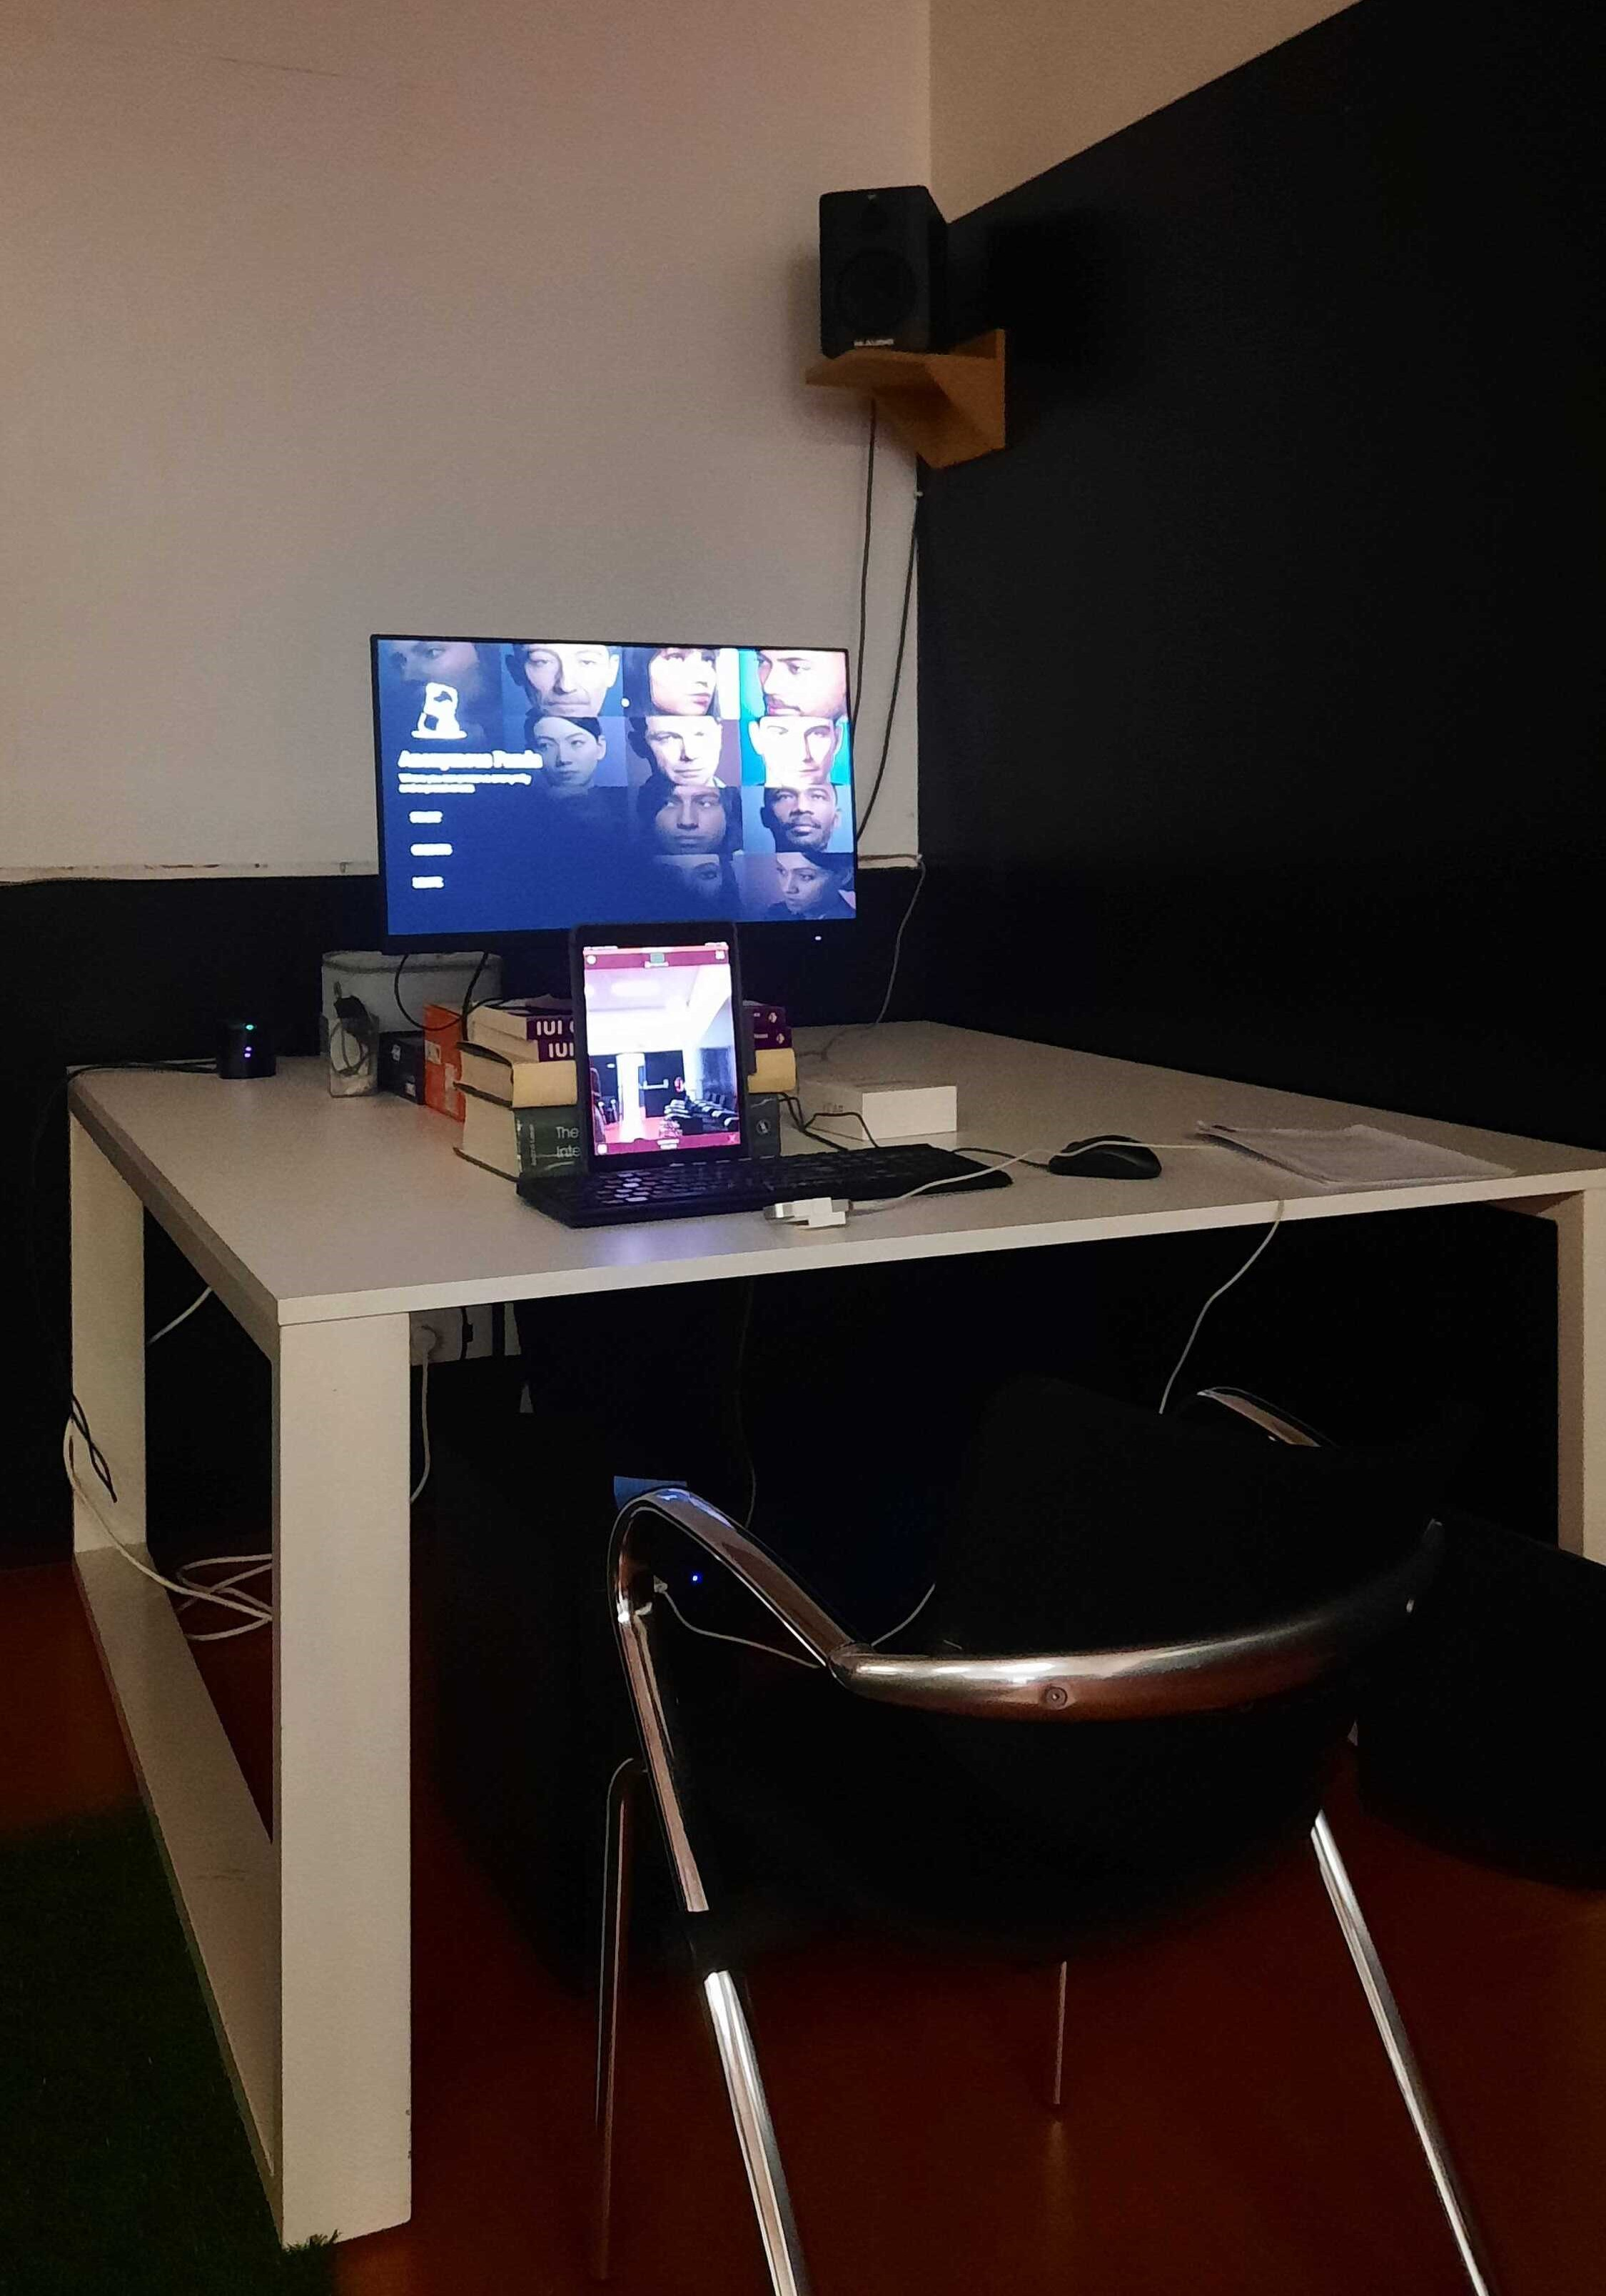
\includegraphics[width=0.84\linewidth]{figures/setup.jpg}
        \captionof{figure}{Room Setup}
        \label{fig:setup}
    \end{minipage}
    \begin{minipage}{0.49\textwidth}
        \centering
        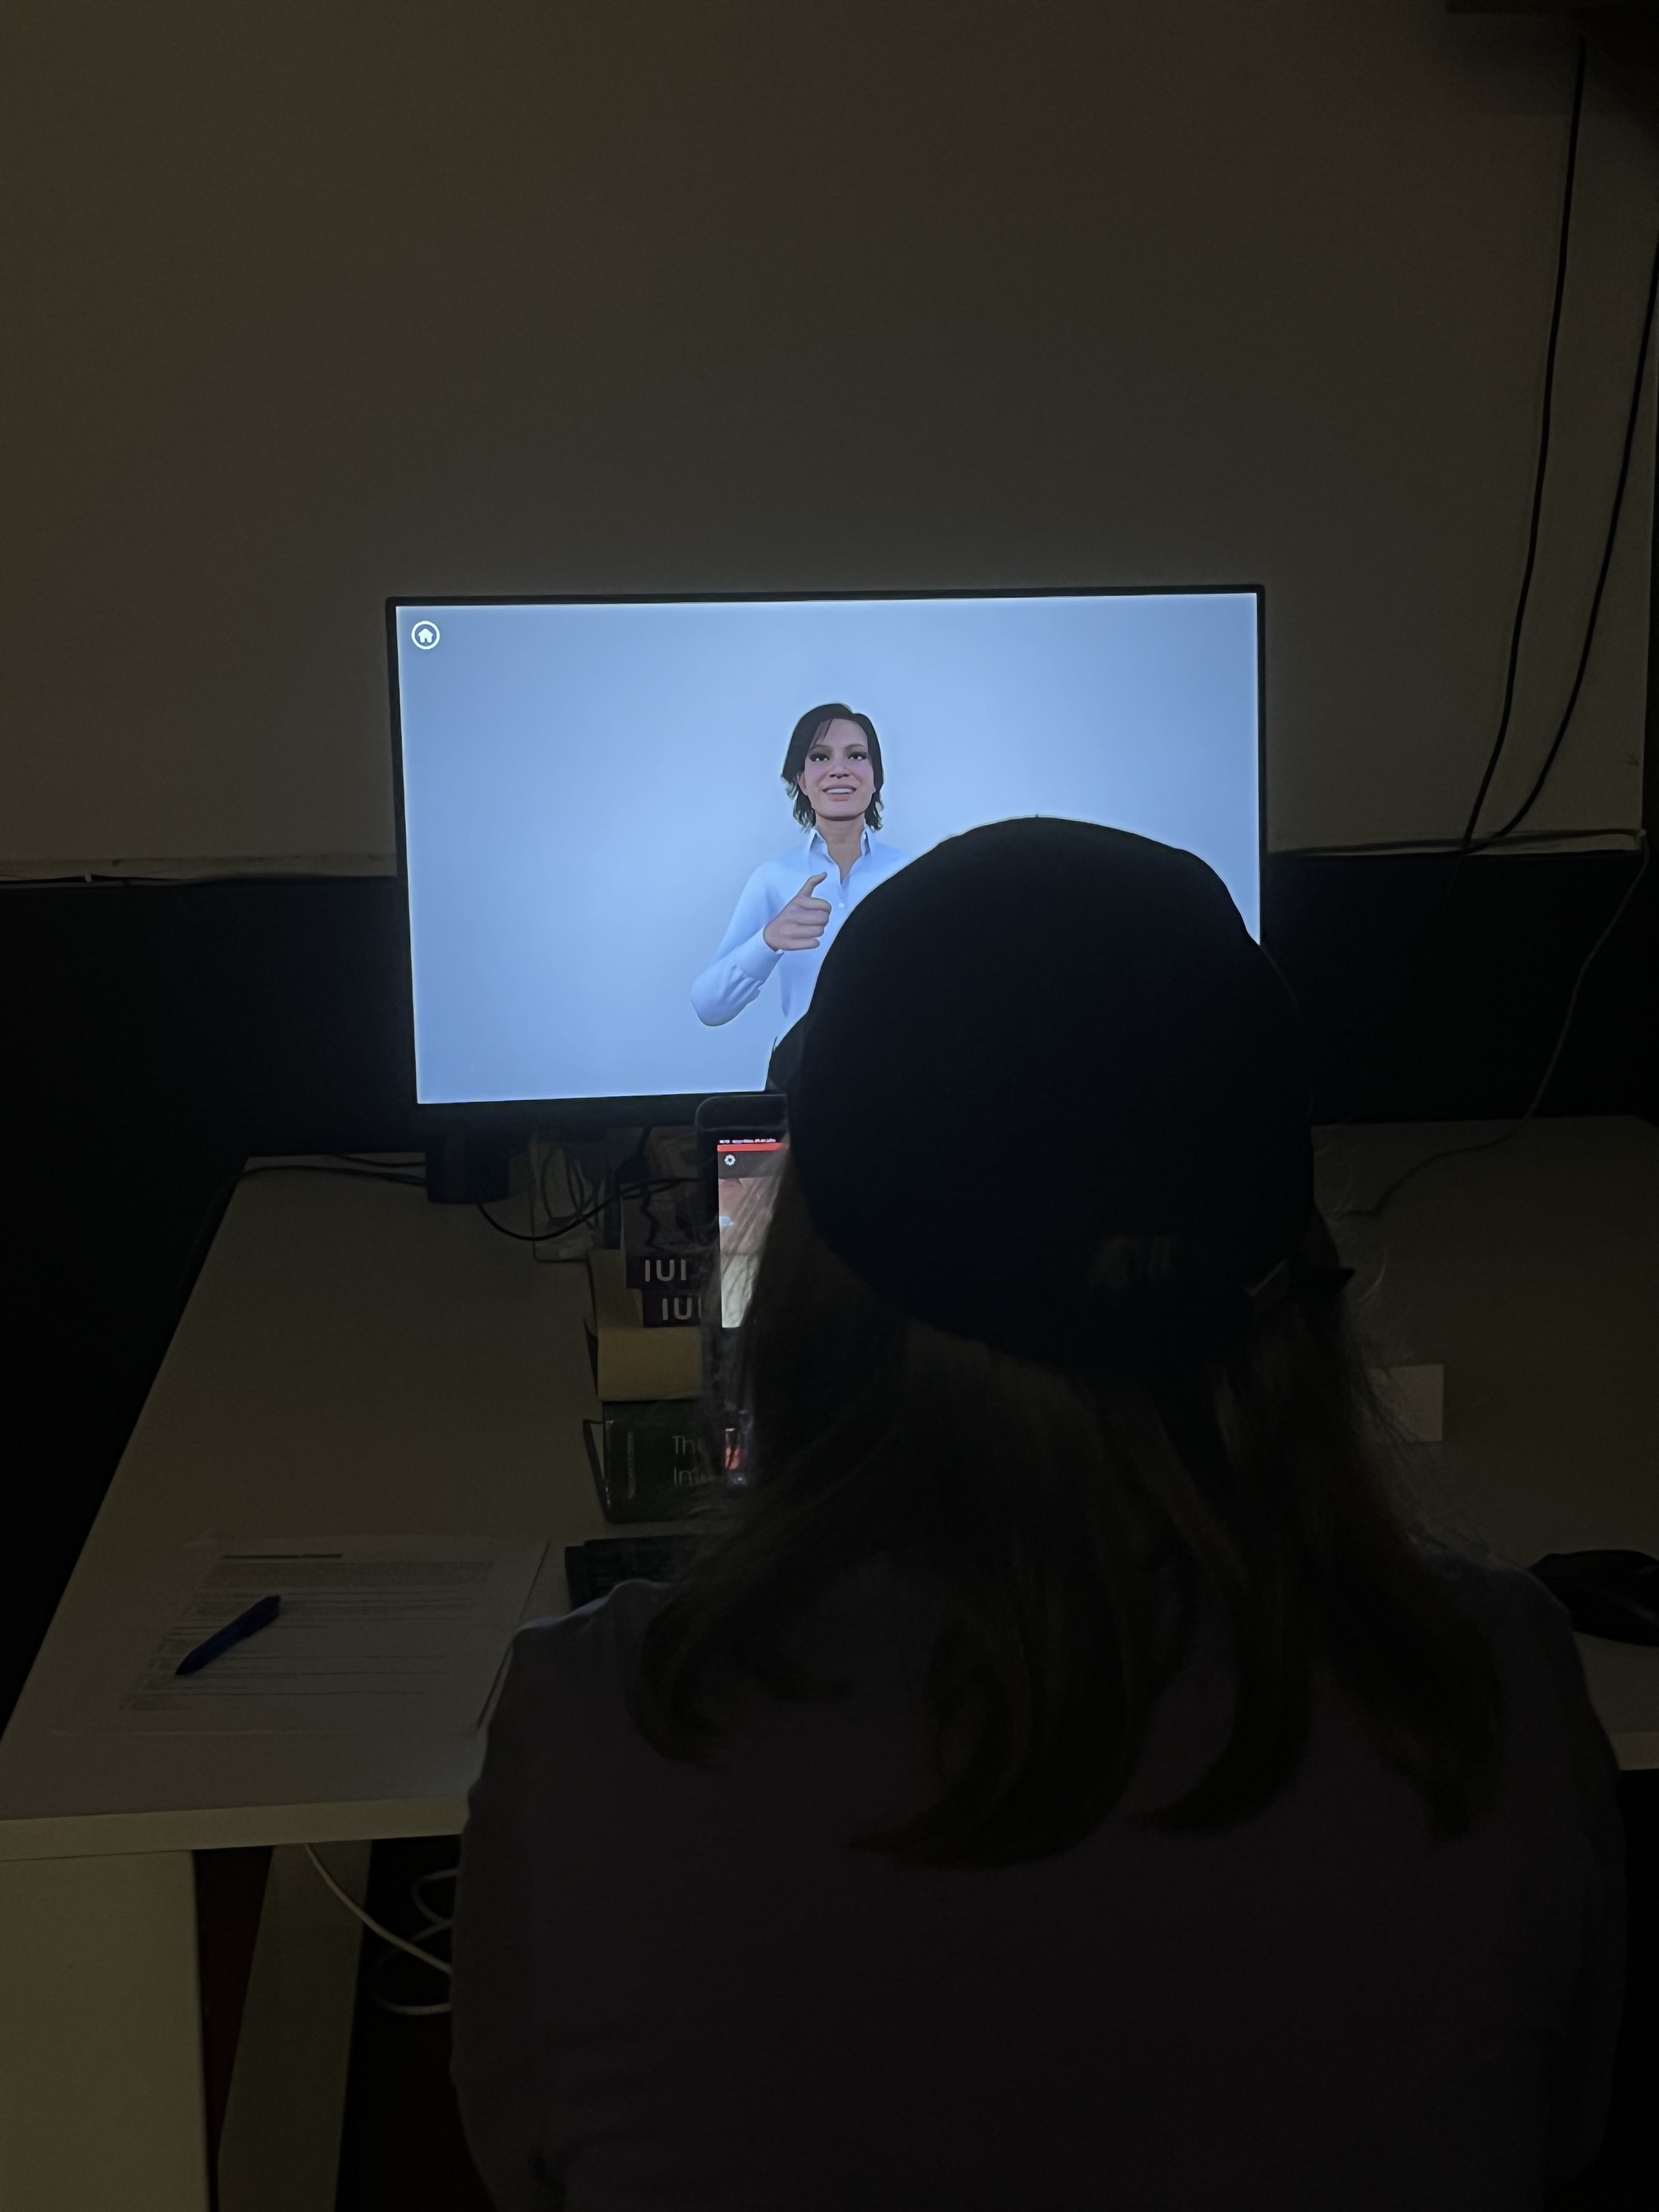
\includegraphics[width=0.9\linewidth]{figures/userTesting.jpg}
        \captionof{figure}{Participant testing our prototype}
        \label{fig:userTesting}
    \end{minipage}
\end{figure}

The participants were then asked to complete a questionnaire designed to assess their perceived anonymity, online public disclosure, perceived usefulness, and perceived ease of use in response to their interaction with our prototype, as proposed by \cite{YUN06, HIT14}.

As mentioned before, for the pre questionnaire (see Appendix \ref{appendix:pre2}) we used five questions to assess the participants' online public disclosure on a seven-point Likert-type scale (1=totally disagree, 7=totally agree), based on the work of Haejin Yun \cite{YUN06}. The five items used to test OPD were: "Usually, I am willing to share my family history and/or secrets", "Usually, I am willing to talk about my failures", "Usually, I am willing to express my most intimate feelings", "Usually, I am willing to talk about my shameful experiences", and "Usually, I am willing to share things I wouldn’t normally share with my family, friends and colleagues".

Regarding the post-questionnaire (see Appendix \ref{appendix:post2}), twenty questions divided into four categories were used, on a seven-point Likert-type scale (1=totally disagree, 7=totally agree), based on the works of Haejin Yun \cite{YUN06} and Hite et al. \cite{HIT14}. Through five questions, each category is responsible for evaluating the participants' perceived anonymity, online public disclosure, perceived usefulness, and perceived ease of use in response to their interaction with our prototype.

Based on the work of Hite et al. \cite{HIT14}, the five questions used to assess the participants' PA were as follows: "While using Anonymous Panda, I am confident others will not know who I am", "While using Anonymous Panda, I think someone may recognize me from my voice", "While using Anonymous Panda, I think someone may recognize me from expressions or words I use frequently", "While using Anonymous Panda, I think someone may find out how old I am", and "While using Anonymous Panda, I am afraid someone will find out who I am". 

The questions used to assess the participants' OPD were similar to those used in the pre questionnaire, but with one minor difference. It asked how the participant felt while using the Anonymous Panda rather than how they normally felt. In other words, we used the pre and post questionnaire questions to see if there was a significant difference in participants' online public disclosure before and after our prototype testing.

The following five items were used to assess the participants' PU: "Using Anonymous Panda would make it easier to express my feelings", "Using Anonymous Panda would increase my willingness to ask for mental health support", "Using Anonymous Panda would enable me to have a more stable mental health quickly", "I think Anonymous Panda can be useful for mental health therapy", and "I feel I am more willing to talk about my problems". PEU was then tested using the following items: "My interaction with Anonymous Panda was clear and understandable", "It was easy to get Anonymous Panda to do what I wanted it to do", "Learning how to use Anonymous Panda was easy for me", "Using Anonymous Panda is intuitive", and "I think Anonymous Panda is easy to use".

Finally, in an open-ended question, participants could express their thoughts on our prototype, as well as what they disliked or thought could be improved. They could also share with us if they used a similar application to ours.

\subsubsection{Hypotheses and Statistical Analyses}
As previously stated, the goal of this study is to put to the test an extended TAM designed to study the user acceptance of the Anonymous Panda. In addition, determine whether virtual avatars can promote interactants' verbal self-disclosure or not (\textbf{RQ\textsubscript{2}}). Therefore, we propose the seven following hypotheses:

\textbf{\textit{H}\textsubscript{1}} - PA has a positive effect on users' acceptance of Anonymous Panda.

\textbf{\textit{H}\textsubscript{2}} - OPD has a positive effect on users' acceptance of Anonymous Panda.

\textbf{\textit{H}\textsubscript{3}} - PU has a positive effect on users' acceptance of Anonymous Panda.

\textbf{\textit{H}\textsubscript{4}} - PEU has a positive effect on users' acceptance of Anonymous Panda.

\textbf{\textit{H}\textsubscript{5}} - PA has a positive effect on OPD.

\textbf{\textit{H}\textsubscript{6}} - PA has a positive effect on PU.

\textbf{\textit{H}\textsubscript{7}} - OPD has a positive effect on PU.

To test \textbf{\textit{H}\textsubscript{1}}-\textbf{\textit{H}\textsubscript{7}}, ...

We also wanted to see if the participants' willingness to provide personal information online altered considerably before and after using the Anonymous Panda application. Due to the fact that participants were measured more than once for the dependent variable, a repeated measures analysis method was required. Therefore, we conducted a Wilcoxon signed-rank test to see whether the participants' willingness to disclose personal information online had changed compared to before they used the Anonymous Panda application. Finally, using a statistical significance level of 0.05, all of this data was evaluated in the IBM SPSS statistics software (v.28, 2021).

\subsubsection{Results}

\begin{figure}[!htb]
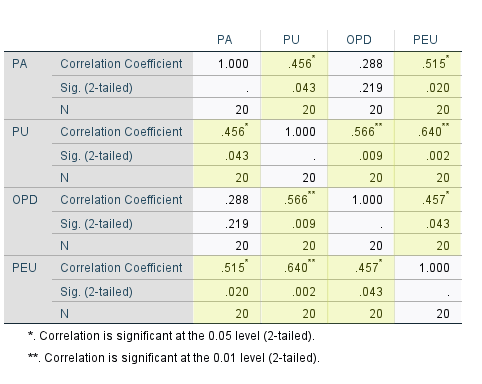
\includegraphics[width=0.8\textwidth]{figures/altCorrelations.png}
\centering
\captionof{table}{Correlations between our variables}
\label{fig:altcorrelations}
\end{figure}

\begin{figure}[!htb]
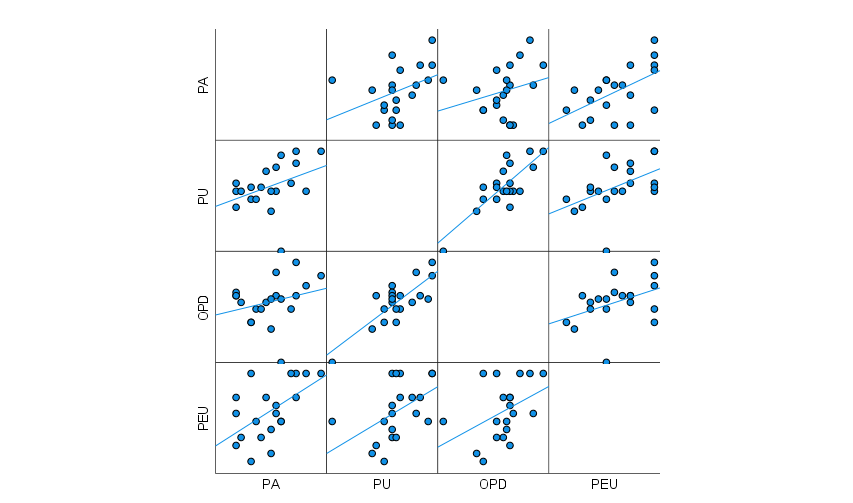
\includegraphics[width=\textwidth]{figures/scatterbox.png}
\centering
\caption{Scatter Plot Matrices}
\label{fig:scatterbox}
\end{figure}

To assess the difference in the participants' willingness to provide personal information online after using the Anonymous Panda app, a Wilcoxon signed-rank test was performed. The results demonstrated a statistically significant improvement in the users' willingness to disclose personal information online following the use of the application (\textit{Z}=-2.543, \textit{p}=.011), with a large effect size (\textit{r}=.57).
 
\subsubsection{Discussion}
% repeated measures to test if there is a statistically significant difference of online public disclosure (OPD) before and after using the anonymous panda app -- Using Wilcoxon signed-rank test

% The results showed a statistically significant positive change in participants' willingness to disclose personal information online after using the anonymous panda app, z=-2.543, p=.011, with a large effect size (r=0.57).
